\documentclass[9pt,twocolumn,twoside,lineno]{biorxiv}
% Use the documentclass option 'lineno' to view line numbers
\setlength{\marginparwidth}{2cm}
\usepackage[textsize=tiny,colorinlistoftodos]{todonotes} % comments in margins
\definecolor{cornflowerblue}{rgb}{0.39, 0.58, 0.93}
\usepackage{blindtext}
\usepackage{gensymb}
\usepackage{amssymb}
\usepackage[switch]{lineno} 
\usepackage{pdfpages}
\usepackage{upgreek}

\def\code#1{\texttt{#1}}

%%%%%%%Add comments in color
\newcommand{\citex}[1]{{\small \textcolor{red}{CITE(#1)}}}
\newcommand{\X}{{\textcolor{red}{X}}}





\newcolumntype{b}{X}
\newcolumntype{s}{>{\hsize=.5\hsize}X}

% Set supplement numbers to S and start counting newly
\newcommand{\beginsupplement}{%
        \setcounter{table}{0}
        \renewcommand{\thetable}{S\arabic{table}}%
        \setcounter{figure}{0}
        \renewcommand{\thefigure}{S\arabic{figure}}%
     }


\title{Teosinte introgression modulates phosphatidylcholine levels and induces early maize flowering time}


\author[a,b,1]{Fausto Rodríguez-Zapata}
\author[a,1]{Allison C Barnes}
\author[b,1]{Karla A Blöcher-Juárez}
\author[c]{Dan Gates}
\author[a]{Andi Kur}
\author[d]{Li Wang}
\author[d]{Garrett M Janzen}
\author[e]{Sarah Jensen}
\author[b]{Juan M Estévez-Palmas}
\author[f]{Taylor Crow}
\author[b]{Rocío Aguilar-Rangel}
\author[g]{Edgar Demesa-Arevalo}
\author[g]{Tara Skopelitis}
\author[b]{Sergio Pérez-Limón}
\author[a, h]{Whitney L Stutts}
\author[a, h]{Peter Thompson}
\author[h]{Yu-Chun Chiu}
\author[g]{David Jackson}
\author[i]{Oliver Fiehn}
\author[f]{Daniel Runcie}
\author[e]{Edward S Buckler}
\author[c]{Jeffrey Ross-Ibarra}
\author[d]{Matthew B. Hufford}
\author[b,j]{Ruairidh JH Sawers}
\author[a, b, *]{Rubén Rellán-Álvarez}

\affil[a]{Department of Molecular and Structural Biochemistry, North Carolina State University, Raleigh, NC}
\affil[b]{National Laboratory of Genomics for Biodiversity, Irapuato, México}
\affil[c]{Department of Evolution and Ecology, Center for Population Biology and Genome Center, University of California, Davis, CA}
\affil[e]{US Department of Agriculture–Agricultural Research Service, Cornell University, Ithaca, NY}
\affil[f]{Department of Plant Sciences, University of California, Davis, CA}
\affil[d]{Department of Ecology, Evolution, and Organismal Biology, Iowa State University, Ames, USA}
\affil[g]{Cold Spring Harbor Laboratory, Cold Spring Harbor, NY, USA}
\affil[h]{Molecular Education, Technology and Research Innovation Center, North Carolina State University, Raleigh, NC}
\affil[i]{West Coast Metabolomics Center, University of California, Davis, CA, USA}
\affil[j]{Department of Plant Science, The Pennsylvania State University, PA, USA}

\keywords{phospholipid metabolism; maize genetics; highland adaptation; convergent evolution}

\runningtitle{\textit{HPC1} selection in highland maize} % For use in the footer 

%% For the footnote.
%% Give the last name of the first author if only one author;
% \runningauthor{FirstAuthorLastname}
%% last names of both authors if there are two authors;
% \runningauthor{FirstAuthorLastname and SecondAuthorLastname}
%% last name of the first author followed by et al, if more than two authors.
\runningauthor{Rodríguez-Zapata, Barnes, Blöcher-Juárez \textit{et al.}}

\begin{abstract}
\section{Abstract}
After domestication from lowland teosinte \textit{parviglumis} (\textit{Zea mays} ssp.\textit{parviglumis}) in the warm Mexican southwest, maize (\textit{Zea mays} ssp. \textit{mays}) colonized the highlands of México and South America. 
In the highlands, maize was exposed to lower temperatures that imposed strong selection on flowering time.
Phospholipids are important metabolites in plant responses to low-temperature, low phosphorus availability and have also been suggested to influence flowering time.

Here, we combined linkage mapping analysis with genome scans to identify \textit{High PhosphatidylCholine 1} (\textit{HPC1}), a gene which encodes a phospholipase A1 enzyme, as a major driver of phospholipid variation in highland maize. 
Common garden experiments demonstrated strong genotype-by-environment interactions associated with variation at \textit{HPC1}, with the highland \textit{HPC1} allele leading to higher fitness in highlands, possibly by hastening flowering. 

The highland maize \textit{HPC1} variant results in impaired function of the encoded protein due to a polymorphism in a highly conserved sequence. 
A meta-analysis indicated a strong association between the identity of the amino acid at this position and optimal growth in prokaryotes. 
Mutagenesis of \textit{HPC1} via genome editing validated its role in regulating phospholipid metabolism. 

Finally, we showed that the highland \textit{HPC1} allele entered cultivated maize by introgression from the wild highland teosinte \textit{Zea mays} ssp. \textit{mexicana} and has been maintained in maize breeding lines from Northern US, Canada and Europe.

Thus, \textit{HPC1} introgressed from teosinte \textit{mexicana} underlies a large metabolic QTL that modulates  phosphatidylcholine levels and has an adaptive effect at least in part via induction of early flowering time.

\end{abstract}

\begin{document}

\maketitle
\thispagestyle{firststyle}
%\marginmark
\firstpagefootnote
\equalcontrib{1}
%\equalcontrib{2}

\correspondingauthoraffiliation{*}{Department of Molecular and Structural Biochemistry, North Carolina State University, 27607, Raleigh, NC. Email: rrellan@ncsu.edu}
\vspace{-33pt}% Only used for adjusting extra space in the left column of the first page

\subsection{Significance Statement}
Despite more than a century of genetic research, our understanding of the genetic basis of the astounding capacity of maize to adapt to new environments is still in its infancy. 
Recent work in many crops has pointed to a potentially important role for introgression in underpinning adaptation, but clear examples of adaptive loci arising via this process are lacking. 
Here, we used an interdisciplinary analysis of the genetic basis of phospholipid metabolism and its role in maize local adaptation to high elevations.
We elucidate the evolutionary history of a novel, major metabolic QTL, that we mapped down to a single gene \textit{HPC1}, and  is the result of a highland teosinte mexicana introgression in maize, which leads to high phosphatidylcholine levels and improves fitness via induction of early flowering. 

\section{Introduction}
%How do organisms adapt to high elevations
Elevation gradients are associated with changes in environmental factors that impose significant physiological constraints on an organism. 
Adaptation to highland environments is achieved via the selection of genetic variants that improve their ability to withstand reduced oxygen availability \cite{Natarajan2016-pc, Yi2010-se, Bigham2010-is, Liu2019-eg}, increased UV radiation \cite{Yang2017-gs} and lower temperatures \cite{Velotta2020-as, Cicconardi2020-gs}.
In particular, low temperatures can significantly reduce the thermal time accumulation to flowering (measured in growing degree days (GDDs) \cite{Gilmore1958-dx} and select for accelerated development and maturity as a compensatory mechanism \cite{Hatfield2015-od}.

%Maize domestication and expansion
Following domestication from teosinte \textit{parviglumis} (\textit{Zea mays} ssp. \textit{parviglumis}) \cite{Matsuoka2002-bg,Piperno2009-fj} in the lowland, subtropical environment of the Balsas River basin (Guerrero, México), cultivated maize (\textit{Zea mays} ssp. \textit{mays}) expanded throughout México and reached the highland valleys of central México around 6,500 years before present \cite{Piperno2001-ea}.

%Contribution of mexicana to highland maize adaptation.
In México, highland adaptation of maize was aided by substantial adaptive introgression from a second subspecies of teosinte, teosinte \textit{mexicana} (\textit{Zea mays} ssp. \textit{mexicana}) that had already adapted to the highlands of México thousands of years after its divergence from teosinte \textit{parviglumis} \cite{Hufford2013-gs, Gonzalez-Segovia2019-jy}. 
Adaptation to low temperature and soils with low phosphorus in highland environments drove \textit{parviglumis} and \textit{mexicana} genetic divergence \cite{AguirreLiguori2019-fl}.
Phenotypically, the most evident signs of \textit{mexicana} introgression into maize are the high levels of stem pigmentation and pubescence \cite{Lauter2004-eq} that are thought to protect against high UV radiation and low temperatures. 
The ability to withstand low temperatures and efficiently photosynthesize during the early stages of seedling development are key factors in maize highland adaptation \cite{Hardacre1980-tq}.
Indeed, recent transcriptome deep sequencing (RNA-seq) analysis showed that the inversion \textit{Inv4m}, introgressed from \textit{mexicana}, strongly affects the expression of genes involved in chloroplast physiology and photosynthesis \cite{Crow2020-gene}.  
\textit{Inv4m} is also associated with earlier flowering times in highland maize \cite{Romero_Navarro2017-cn, Gates2019-xu}. 
Given the low accumulation of growing degree days in typical highland environments, selection has favored shorter generation  times in highland adapted maize \cite{Gates2019-xu}.
By the time maize reached the Mexican highlands, its range had already expanded far to the South, including colonization of highland environments in the  Andes \cite{Athens2016-ep, Grobman2012-pm}. 
Andean maize adaptation occurred without \textit{mexicana} introgression, as there is no known wild teosinte relative in South America.
These multiple events of maize adaptation to highland environments make maize a good system to study the evolutionary and physiological mechanisms of convergent adaptation \cite{Takuno2015-uj, Wang2020-mp}.

%Photoperiod adaptation
In comparison to its southward expansion, the northward migration of maize into modern-day United States, where summer daylengths are longer, occurred at a much slower pace \cite{Da_Fonseca2015-zh, Swarts2017-ge} due to delayed flowering of photoperiod-sensitive tropical maize lines \cite{Hung2012-ms}.
Indeed, a host of evidence suggests that maize cultivation in northern latitudes was enabled by the selection of allelic variants that led to a reduction in photoperiod sensitivity to allow flowering under longer photoperiods \cite{Liang2018-af, Guo2018-on, Coles2010-db, Huang2018-ga, Yang2013-lg, Salvi2007-ku, Hung2012-ms}.
Some of the early flowering alleles that conferred an adaptive advantage in highland environments are the result of \textit{mexicana} introgressions into highland maize \cite{Guo2018-on} that were further selected at northern latitudes.
Photoperiod-insensitive maize from the Northern US and Canada thrived when introduced into Northern Europe, as it was already pre-adapted to northern latitudes and lower temperatures \cite{Brandenburg2017-ii}.
Introgression of highland-adapted teosinte \textit{mexicana} into highland maize can be a critical source of adaptive genetic variation for modern maize adapted to high latitudes.
However, genetic, physiological and phenotypic evidence of such events is  limited.

Plant phospholipids, as well as other glycerolipids such as sulfolipids, galactolipids and less polar lipids such as triacylglycerols, are involved in plant responses to low temperature.
Phospholipid levels are increased in plants exposed to low temperatures \cite{Degenkolbe2012-wf} and levels of unsaturated fatty acids in glycerolipids are reduced \cite{Welti2002-uk, Lynch1987-ln}, which may help maintain the fluidity of cell membranes.
Under stressful conditions, the proportions of differently shaped lipids in plants are modulated to maintain membrane flexibility while preventing membrane leakage. 
For instance, phosphatidylcholines (PCs) are rectangular polar lipids that are well suited for the formation of bilayer membranes because the size of their glycerol backbone, choline headgroup and fatty acid tails are similar.
By contrast, lyso-phosphatidylcholine (LPC) is a triangular PC with a single acyl group that cannot form a bilayer because its headgroup is much larger than its fatty acid \cite{Jouhet2013-fv}.
LPCs do allow for some membrane movement, but high LPC concentrations act as a detergent \cite{Henriksen2010-cm} and can facilitate cell leakage and damage at low temperatures, effects that would be prevented by higher PC levels.
In cold-adapted maize temperate lines and \textit{Tripsacum} species (a distant maize relative), genes involved in  phospholipid biosynthesis show accelerated rates of protein sequence evolution, further supporting an important role for phospholipid metabolism across several species during cold adaptation \cite{Yan2019-tx}. 
Finally, certain species of PC, the most abundant phospholipid  in plant cells \cite{Gu2017-nd}, can bind to \textit{Arabidopsis thaliana} FLOWERING LOCUS T (FT) and accelerate flowering through an unknown mechanism \cite{Nakamura2014-qf}. 
Consistent with this observation, glycerolipid levels in maize have predictive power for flowering time \cite{Riedelsheimer2013-bd}. 

Here, we identified an adaptive teosinte \textit{mexicana} introgression that alters highland maize phospholipid metabolism and leads to early flowering.
Using genome scans and linkage mapping, we identified \textit{High PhosphatidylCholine1} (\textit{HPC1}), encoding a phospholipase A1, as a driver of high PC levels in highland maize. 
Data from thousands of genotyped landrace test-crosses grown in common garden experiments at different elevations in México showed a strong genotype-by-environment effect at the \textit{HPC1} locus, where the highland allele leads to higher fitness in the highlands and reduced fitness at lower elevations.
Furthermore, we determined that the highland \textit{HPC1} allele that was introgressed from teosinte \textit{mexicana} was carried northward and is now present in maize cultivars grown in the Northern US and European Flint lines.
These results suggest that the \textit{HPC1} highland allele has a beneficial effect in cold, high-latitude environments, where early flowering is advantageous.

\section{Results}
\label{sec:results}
\subsection{Highland Mesoamerican landraces show high PC/LPC ratios and selection of highly unsaturated PCs}
We grew a diversity panel composed of 120 highland and lowland landraces from Mesoamerica and South America (Figure \ref{Fig1}A, Sup. File 1), hereafter referred to as the HiLo diversity panel, in highland and lowland Mexican common gardens and quantified glycerolipid levels.    
We observed that Mesoamerican highland landraces have  high PC/LPC ratios,  particularly when grown in the highlands (Figure \ref{Fig1}B).
The differences observed in phospholipid levels between highland and lowland maize may be the result of adaptive natural selection or random genetic drift during the process of maize colonization of highland environments.
To distinguish between these two competing possibilities, we compared the variance of each phenotype across the population with the genetic variance of neutral markers, using a $Q_{ST}$-$F_{ST}$ comparison \cite{Leinonen2013-ic}.
We calculated $Q_{ST}$-$F_{ST}$ using DartSeq genotypic data from the same plants that were used to analyze glycerolipid levels, and calculated the $Q_{ST}$-$F_{ST}$ values for each glycerolipid species for highland/lowland populations from each continent. 
Mean $Q_{ST}$ was greater than mean $F_{ST}$ in Mesoamerican and South American comparisons, although only the Mesoamerican comparison was significant (two-tailed \textit{t}-test, $p$ = 0.00073; South American comparison $p$ = 0.12).
However, we noticed several PC and LPC species with higher $Q_{ST}$ values than the neutral $F_{ST}$ in both continents (Figure \ref{Fig1}C-D).
The species with the highest $Q_{ST}$ value in both continents was PC-36:5. 
In summary, highland Mesoamerican landraces grown in highland conditions had particularly high PC/LPC ratios and levels of PC species, especially of species with high levels of unsaturation (e.g., PC-36:5). 

\subsection{Genes involved in PC/LPC conversion show strong highland selection signals} 
We used genotyping by sequencing (GBS) data from 2,700 Mexican maize landraces, generated by the SeeD project \cite{Romero_Navarro2017-cn, Gates2019-xu}, to run a principal component-based (\textit{pcadapt}) analysis to determine how loci might contribute to observed patterns of differentiation between major principal components of genetic variation \cite{Luu2017-ws}.
The first principal component of \textit{pcadapt} separated Mexican landraces based on the elevation of their geographical origin (\ref{SupFig1}A).
Using this first principal component, we identified outlier SNPs across the genome that are significantly associated with landrace elevation and potentially involved in local adaptation (\ref{SupFig1}B).
We independently catalogued $\approx 600$ maize genes known to be involved in glycerolipid metabolism (See Materials and Methods for details). From those, 85 contained single nucleotide polymorphisms (SNPs) that were \textit{pcadapt} PC1 outliers (top 5\% -log(P)) (Sup. File 2).
\begin{figure}[hbp]
\begin{center}
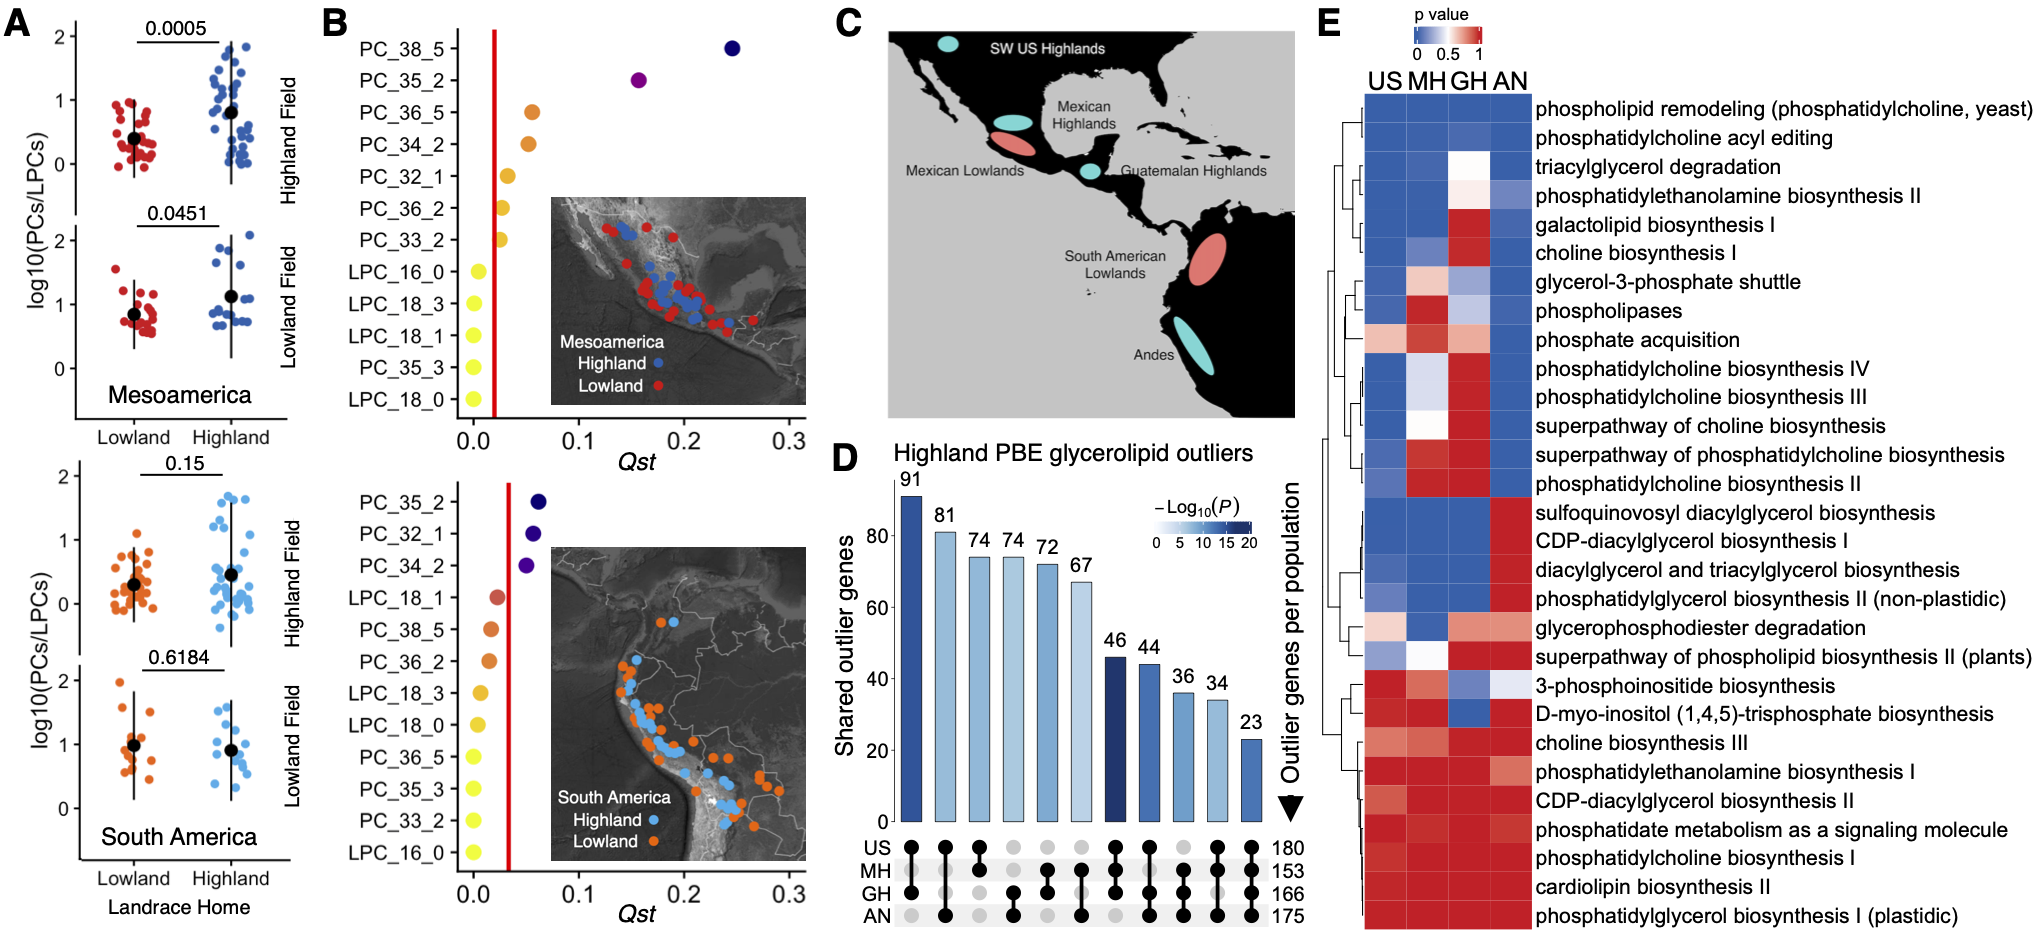
\includegraphics[width=0.4\paperwidth]{Figures/Fig_1.png}
\caption{\textbf{Phospholipid selection in highland maize.} 
\textbf{A)} Map showing the geographical origin of the 120 maize accessions from the HiLo diversity panel used in the common garden experiment to quantify glycerolipid levels.
\textbf{B)} PC/LPC ratio, in log\textsubscript{10} scale, of highland and lowland landraces from Mesomerica and South America; adjusted pairwise comparison \textit{t}-test \textit{p}-values are shown.
\textit{$Q_{ST}$-$F_{ST}$} analysis of phospholipid compounds between highland and lowland landraces from Mesoamerica \textbf{C)} and South America \textbf{D)}.
} 
\label{Fig1}
\end{center}
\end{figure}

\begin{figure*}[ht]
\begin{center}
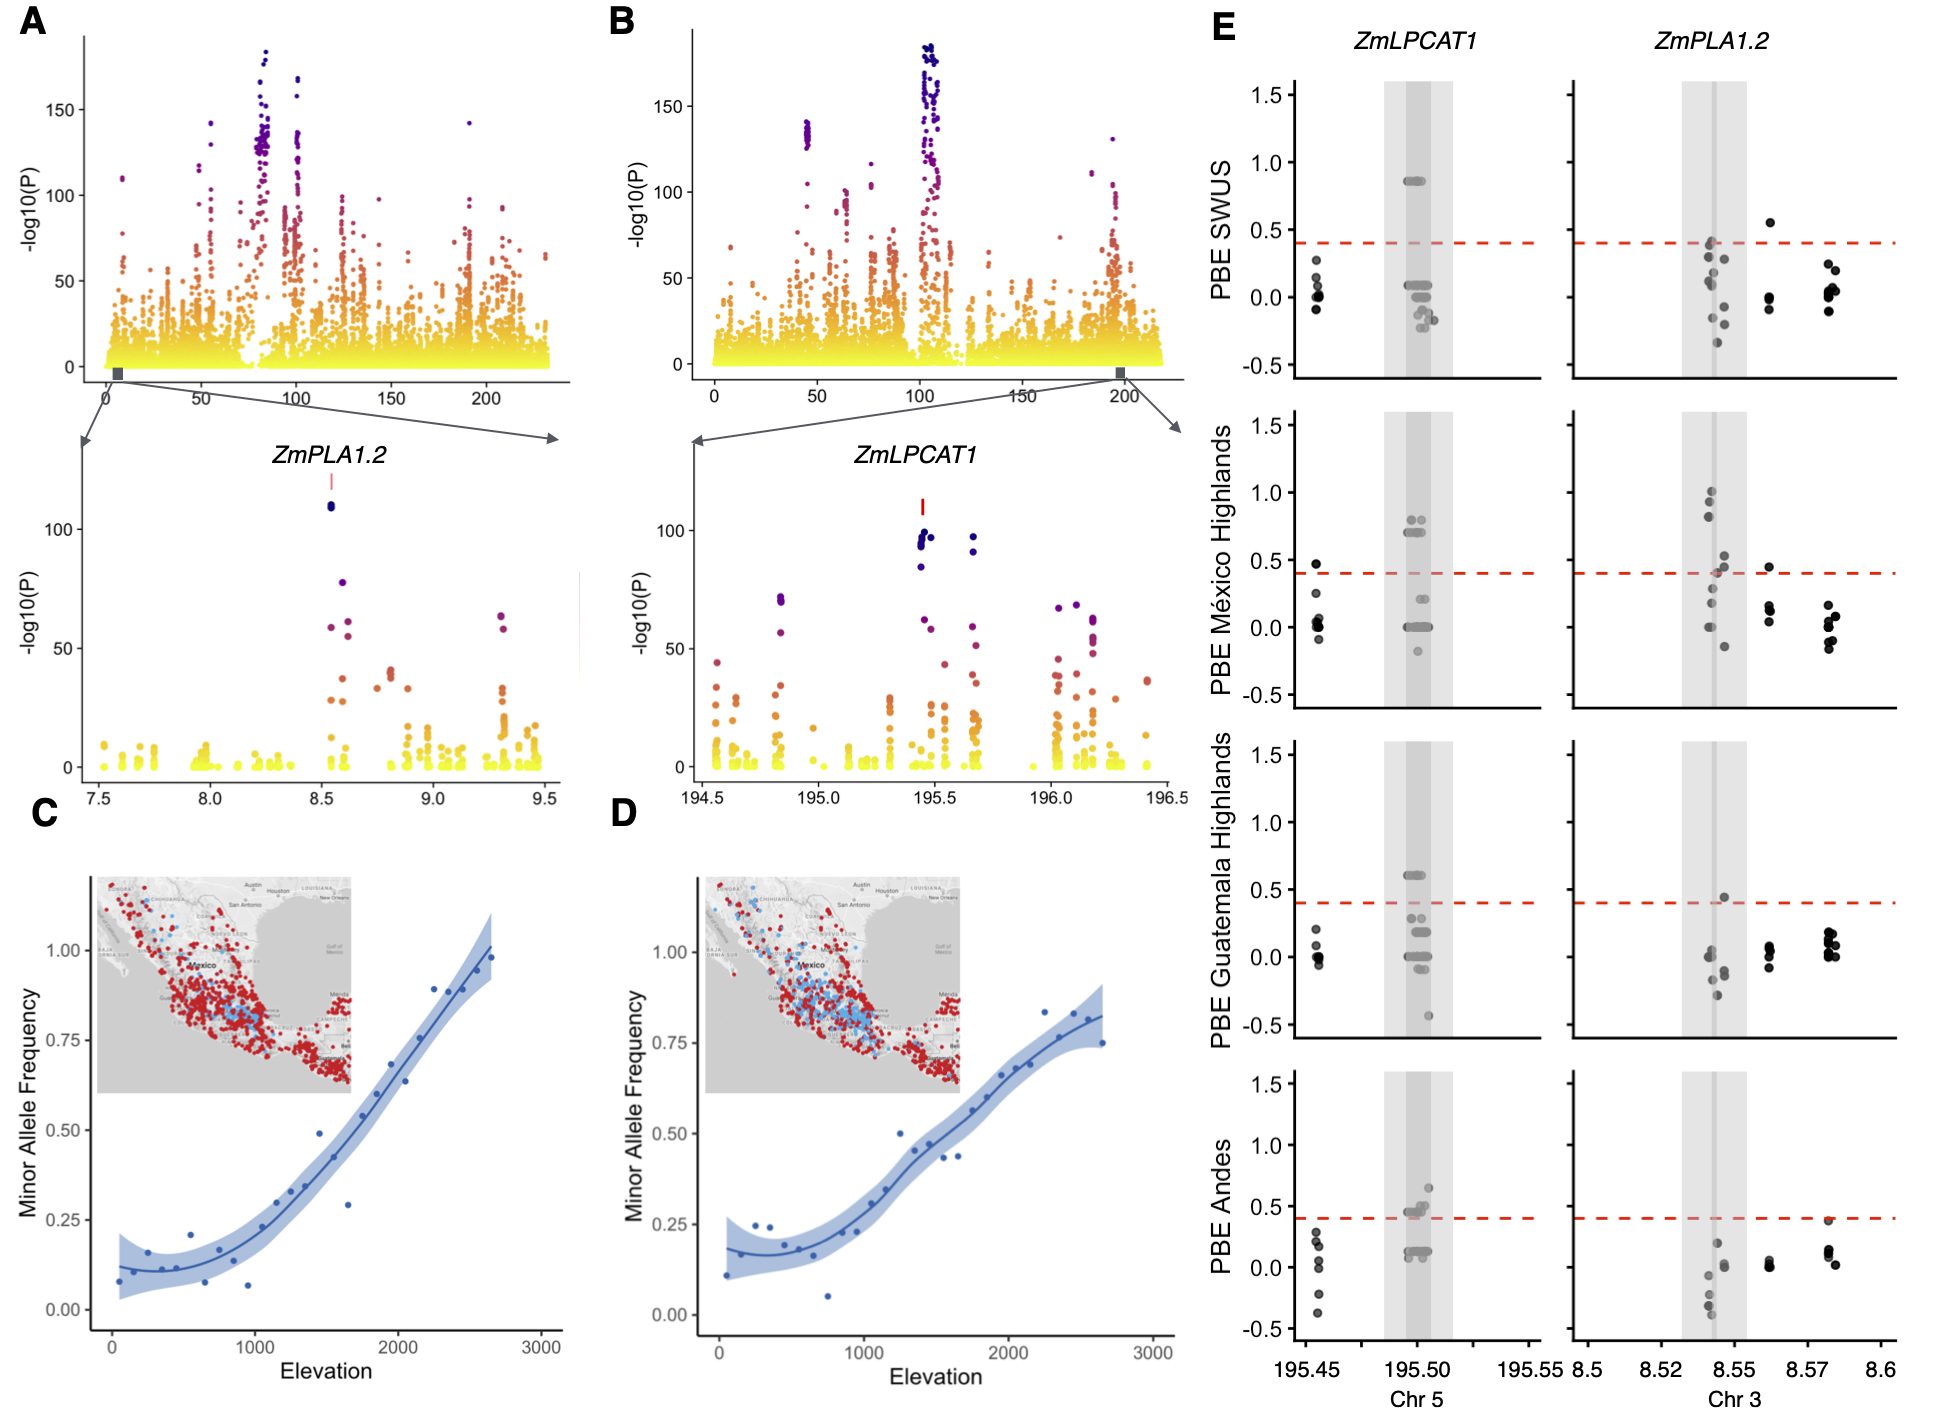
\includegraphics[width=0.6\paperwidth]{Figures/Fig_2.png}
\caption{\textbf{Evidence of highland selection in genes determining PC/LPC ratios.}
Manhattan plots of minus log\textsubcript{10}(p‐values) \textit{pcadapt} outliers. 
\textbf{A)} and \textbf{B)} \textit{pcadapt} PC1 outlier plots of chromosomes 5 and 3, respectively. 
Lower panels zoom in on areas of outlier SNPs that co-localize with the physical position of the coding sequences (marked with a red vertical line) of \textit{HPC1} and \textit{ZmLPCAT1}. 
\textbf{C)} and \textbf{D)} the geographic- and elevation-dependent minor allele frequencies of the highland (blue) and lowland (red) alleles of one of the outlier SNPs in the coding sequence of \textit{HPC1} and \textit{ZmLPCAT1}.
\textbf{E)} PBE values of SNPs in \textit{ZmLPCAT1} and \textit{HPC1}.} 
\label{Fig2}
\end{center}
\end{figure*}

\begin{figure*}[!ht]
\begin{center}
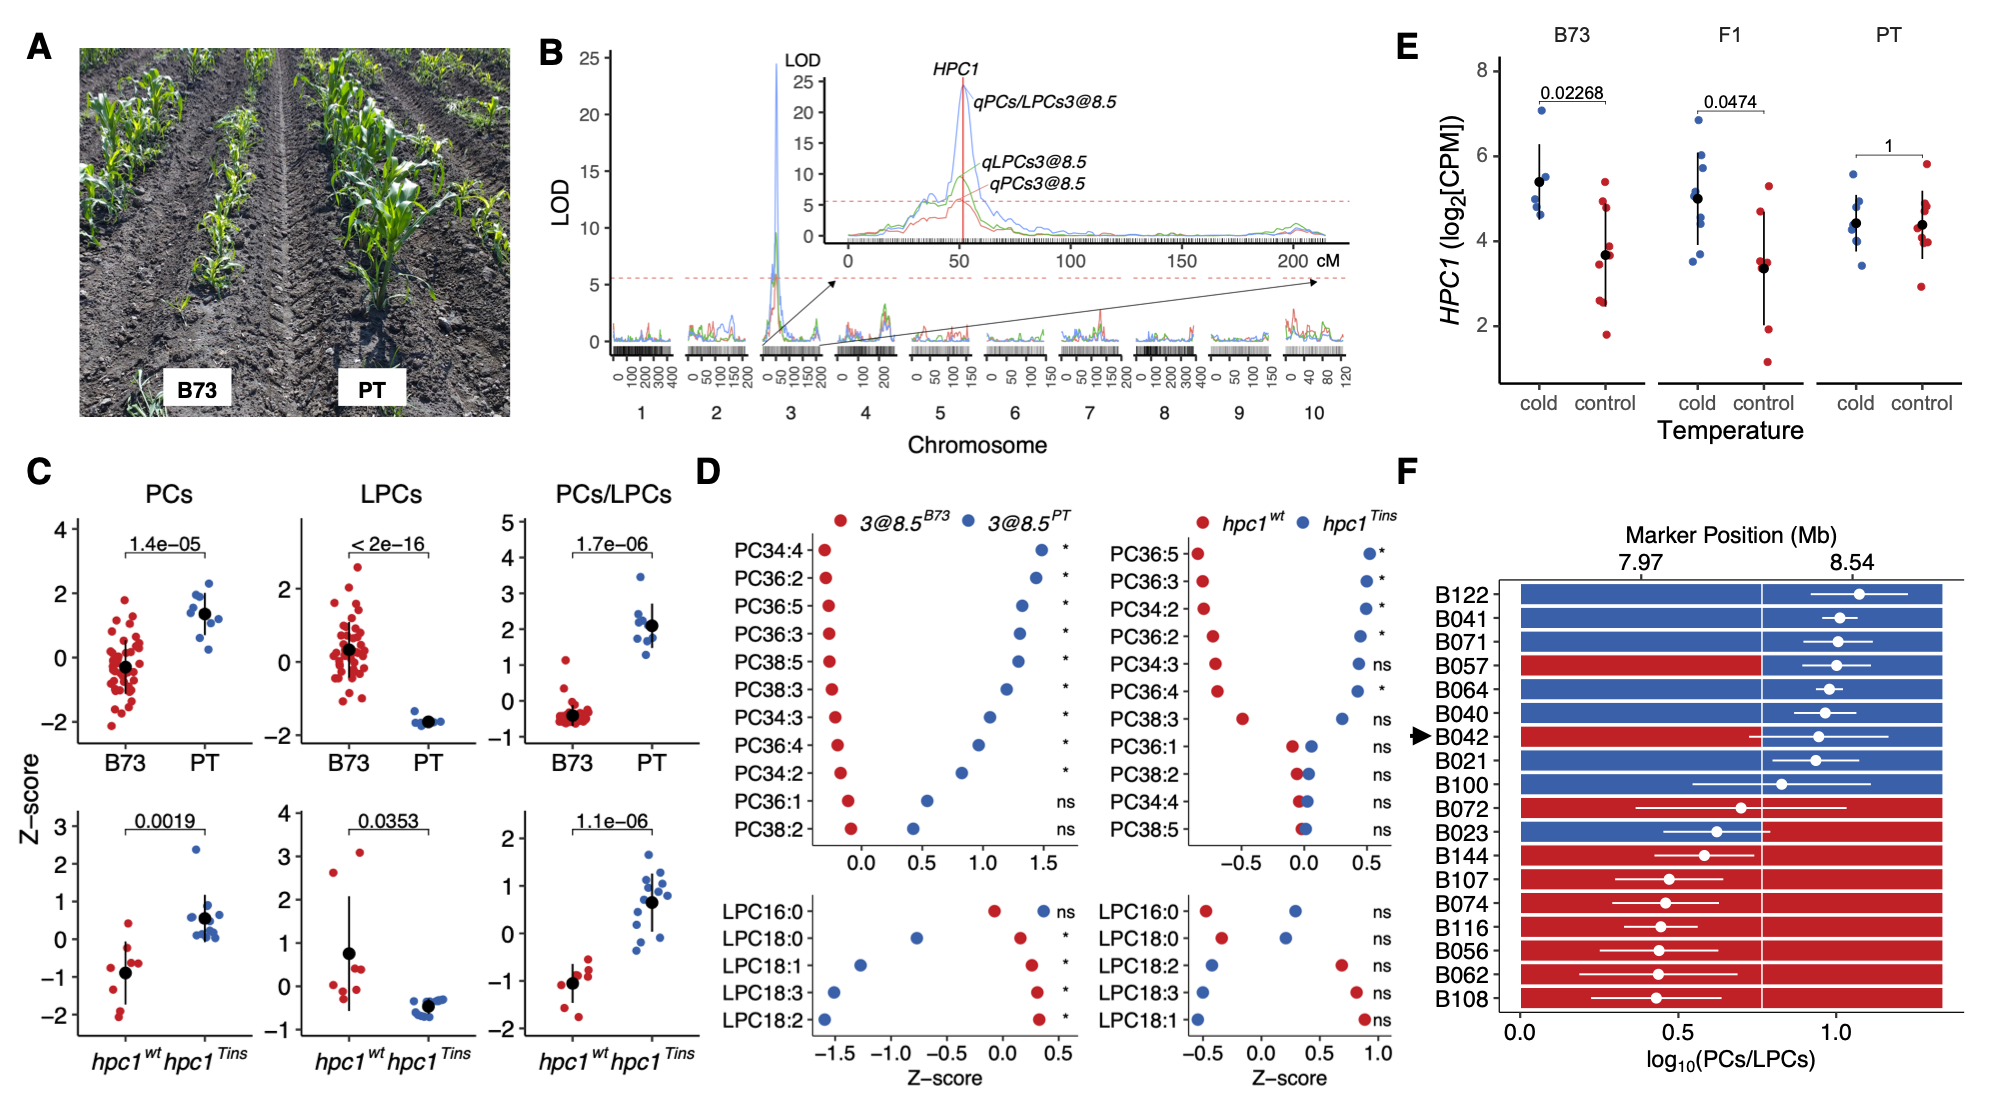
\includegraphics[width=0.8\paperwidth]{Figures/Fig_3.png}
\caption{\textbf{\textit{HPC1} defines a major QTL explaining PC/LPC conversion.} 
\textbf{A)} PT and B73 plants growing in the highland Metepec field. 
\textbf{B)} QTL analysis using data collected from plants growing in the highland and lowland fields for PC and LPC levels and the PC/LPC ratio identified overlapping major QTLs at 8.5 Mb on chromosome 3. 
The QTL peaks coincide with the physical location of \textit{HPC1}. 
\textbf{C)} Effect sizes for PCs, LPCs and PC/LPCs (z-score normalized) in RILs at 8.5 Mb on chromosome 3 that are either homozygous for B73 or PT (top row) and CRISPR-Cas9 \textit{hpc1\textsuperscript{CR}} mutant and wild-type plants (bottom row).        
\textbf{D)} Effect sizes for individual PC and LPC species (z-score normalized) in RILs at 8.5 Mb on chromosome 3 (top row) and CRISPR/Cas9 \textit{hpc1\textsuperscript{CR}} mutant.
\textbf{E)} \textit{HPC1} expression analysis in B73, PT and their F\textsubscript{1} hybrids grown in standard and cold temperatures in a growth chamber.
\textbf{F)}PC/LPC ratio for several RILs. RIL B042 (indicated by the black arrow) bears a recombination event 500 bp upstream of the \textit{HPC1} translation start codon.
In panels C-F, phenotypes associated with the B73 haplotype are in red; the equivalent values for the PT haplotype are in blue.}
\label{Fig3}
\end{center}
\end{figure*} 
The genes  \textit{High PhosphatidylCholine 1} (\textit{HPC1}, \textit{Zm00001d039542}) and \textit{Lyso-Phosphatidylcholine Acyl Transferase 1} (\textit{ZmLPCAT1}, \textit{Zm00001d017584}), which are involved in phospholipid remodeling, had SNPs within their coding sequence with significantly high -log(P) values (Figure \ref{Fig2}A-B), indicating strong elevation-dependent allele frequency changes (Figure \ref{Fig2}C-D). 
We then used the same set of 600 glycerolipid metabolism-related genes to identify selection signals using the Population Branch Excess (PBE) \cite{Pool2017-oa} statistic across four highland populations: Southwestern US (SWUS), Mexican Highlands (MH), Guatemalan Highlands (GH) and Andes \cite{Wang2020-mp}.
We established that, of the 153 glycerolipid-related genes that were PBE outliers in the Mexican Highlands, 38 were also \textit{pcadapt} PC1 outliers (Sup. File 2).
%Hufford: statistically  more overlap than expected?
There are two possible explanations for the extent of convergent selection in highland populations (see \cite{Wang2020-mp, yeaman2018}). 
Adaptation may be conferred by a small number of genes, thereby imposing a \textit{physiological} constraint on the sources of adaptation leading to convergence. 
Alternatively, adaptation may be the result of many genes, but deleterious \textit{pleiotropic} effects restrict the number of genes that can be targeted by selection, also leading to convergence.  
Using Yeaman's \textit{et al.} $C_{hyper}$ statistic \cite{yeaman2018}, which quantifies these two modes of convergent adaptation, we determined that the overlap among putative adaptive genes in the four highland populations cannot be explained merely by physiological constraints ($C_{hyper} = 3.96$). A certain degree of pleiotropic constraint is therefore likely.
Overlap between adaptation candidates was higher for the SWUS MH and GH population pairs ($C_{hyper} = 4.79$) than between the Andean and SWUS MH and GH pairs ($C_{hyper} = 3.14$).
We identified a significant excess of genes that are targets of selection in more than two populations ($P< 3 \times 10^{-5}$, \ref{SupFig1}C).
The most over-represented intersection of selected glycerolipid genes was in the SWUS, MH and GH populations ($p = 1  \times 10 ^{-15} $, \ref{SupFig1}C), perhaps indicating a set of genes specifically selected in this geographical region relative to the Andean material and/or closer kinship between those populations and thus weaker statistical independence.
From the glycerolipid pathways, 22 genes were PBE outliers consistently across all four populations ($p =<1  \times  ^{-10}$, \ref{SupFig1}C). 
We then performed an independent analysis for each of the 30 glycerolipid metabolism pathways and compared their average PBE value (using a 10-kb window around each constituent gene)  with a genome-wide genic random sampling distribution of PBE values. 
The pathways related to 'phospholipid remodeling'  and 'PC acyl editing' had significantly higher PBE values in all four populations, indicating a possible role for phospholipid remodeling in maize highland adaptation (\ref{SupFig1}D and Sup. File 2). 
For example, \textit{ZmLPCAT1} is a selected gene  in the 'phospholipid remodelling' and 'PC acyl editing' pathways with shared outlier SNPs in the coding sequence region across all four populations (Figure \ref{Fig2}E, Sup. File 2). 
HPC1 performs the reverse reaction of ZmLPCAT1 and is part of the 'PC acyl editing', 'triacylglycerol degradation' and 'phospholipases' pathways. 
\textit{HPC1} displayed particularly high PBE values in the Mexican Highland population and contained SNPs that are unique to each population and others that are shared across populations (Figure \ref{Fig2}E). 
Together, we showed here using two independent datasets that pathways involved in phospholipid remodelling and in particular two genes (\textit{HPC1} and \textit{ZmLPCAT1}) controlling the PC/LPC ratio show strong selection signals in highland maize.

\begin{figure}[!ht]
\begin{center}
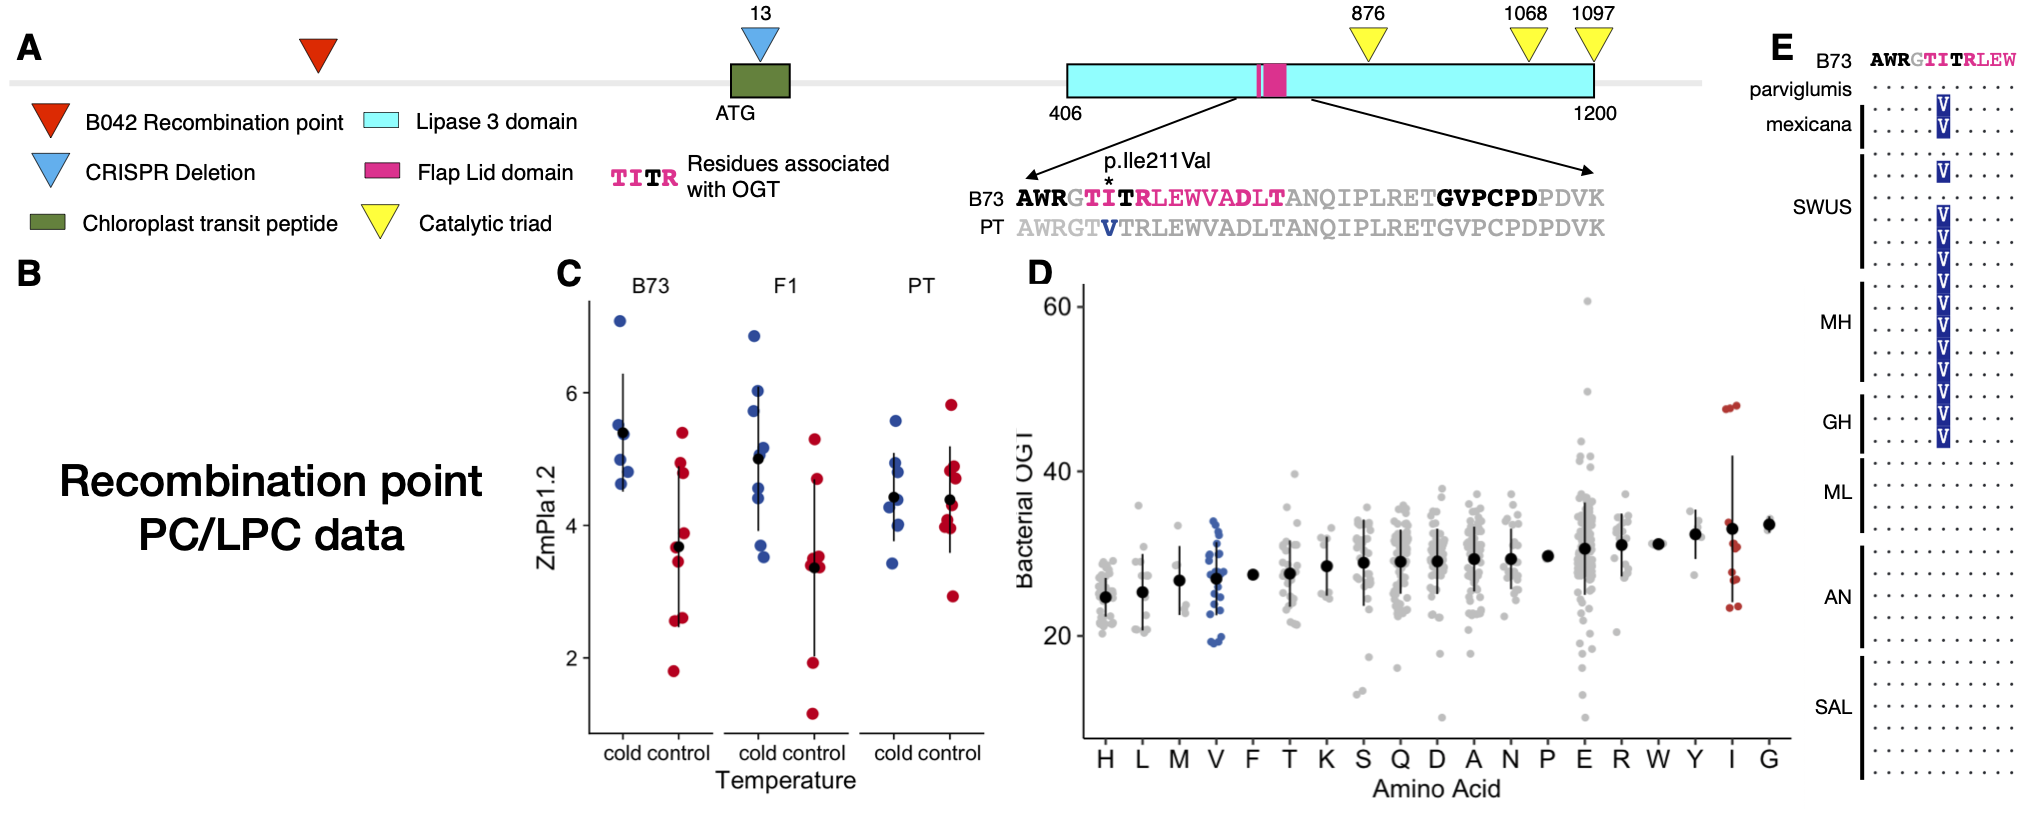
\includegraphics[width=0.4\paperwidth]{Figures/Fig_4.png}
\caption{\textbf{Fitness effects of the \textit{HPC1-PT} allele} 
We used best linear unbiased predictions (BLUPs) and GBS data from 2,700 landraces from \cite{Gates2019-xu}, evaluated in 23 common gardens at different elevations in México. 
We modeled each trait as a function of the \textit{HPC1-PT} genotype, trial elevation, and tester line, with controls for main effects and responses to elevation of the genomic background. 
Gray lines and ribbons show estimates of the effect of the highland allele of \textit{HPC1-PT} as a function of common garden elevation ± 2 standard errors of the mean, using the \textit{GridLMM} package \cite{Runcie2019-Gr}. 
Purple lines show estimates of the \textit{HPC1-PT} effect in a model that also includes effects of days to anthesis. ASI, anthesis to silking interval.}
\label{Fig4}
\end{center}
\end{figure}

\subsection{A major QTL explaining PC to LPC conversion overlaps with \textit{HPC1}} 
To break population structure and identify loci involved in phospholipid biosynthesis in highland maize, we developed a recombinant inbred line (RIL) BC1S5 population derived from a cross between the temperate inbred line B73 and the Mexican highland landrace Palomero Toluqueño (PT), using B73 as the recurrent parent (75\% B73, 25\% PT). 

The parental PT accession is a popcorn landrace (palomero means popcorn in Spanish) from the Toluca Valley in México (\textit{Mexi5} CIMMYTMA 2233) (Figure \ref{Fig3}A). 
We grew the Hilo diversity panel and the B73 x PT BC1S5 mapping population in the same highland and lowland common gardens and collected samples for glycerolipid analysis.
The locally adapted PT landrace showed higher fitness than B73 in the highland field (Figure \ref{Fig3}A), probably due to adaptation to low temperatures in this highland environment.  
In the Mexican highlands, values of around 5 GDD are typical, while 15-20 GDD are common in lowland environments. 
We detected major quantitative trait loci (QTLs) for the sum of LPC species levels, PC species levels and the PC/LPC ratio that all mapped to the same locus on chromosome 3, at around 8.5 Mb (Figure \ref{Fig3}B). 
The PC/LPC ratio QTL had the highest logarithm of the odds (LOD) score, i.e., 24.5, and explained the most phenotypic variance (87\%). 
We searched for evidence of epistatic interactions for LPC levels, PC levels, and the PC/LPC ratio through a combination of R/qtl \code{scantwo} and \code{stepwise} functions \cite{Broman2003-ac}, but identified none.
The three QTLs \textit{qLPCs3@8.5}, \textit{qPCs3@8.5} and \textit{qPCs/LPCs3@8.5} were robust against environmental effects and were detected in both the highland and lowland environments.
The additive effect of the PT allele at these QTLs was associated with high levels of PCs, low levels of LPCs and consequently high PC/LPC ratios, while the B73 allele had the opposite effect (Figure \ref{Fig3}C, top panel).
Individual QTLs for PC and LPC species at this locus showed the same additive effect for the PT allele as the sum of each class of species (from the QTLs \textit{qPCs@8.5} and \textit{LPCs3@8.5}) (Figure \ref{Fig3}C, top panel and \ref{SupFig2}). 
All individual LPC QTLs at the \textit{qLPCs3} locus corresponded to LPCs that contain at least one double bond in their fatty acid (\ref{SupFig2}, Sup. file 3).
\textit{qPCs3@8.5} was driven mainly by PC species with more than two fatty acid double bonds, such as PC 36:5 (Figure \ref{Fig3}D and \ref{SupFig2} bottom panel).

\begin{figure*}[!ht]
\begin{center}
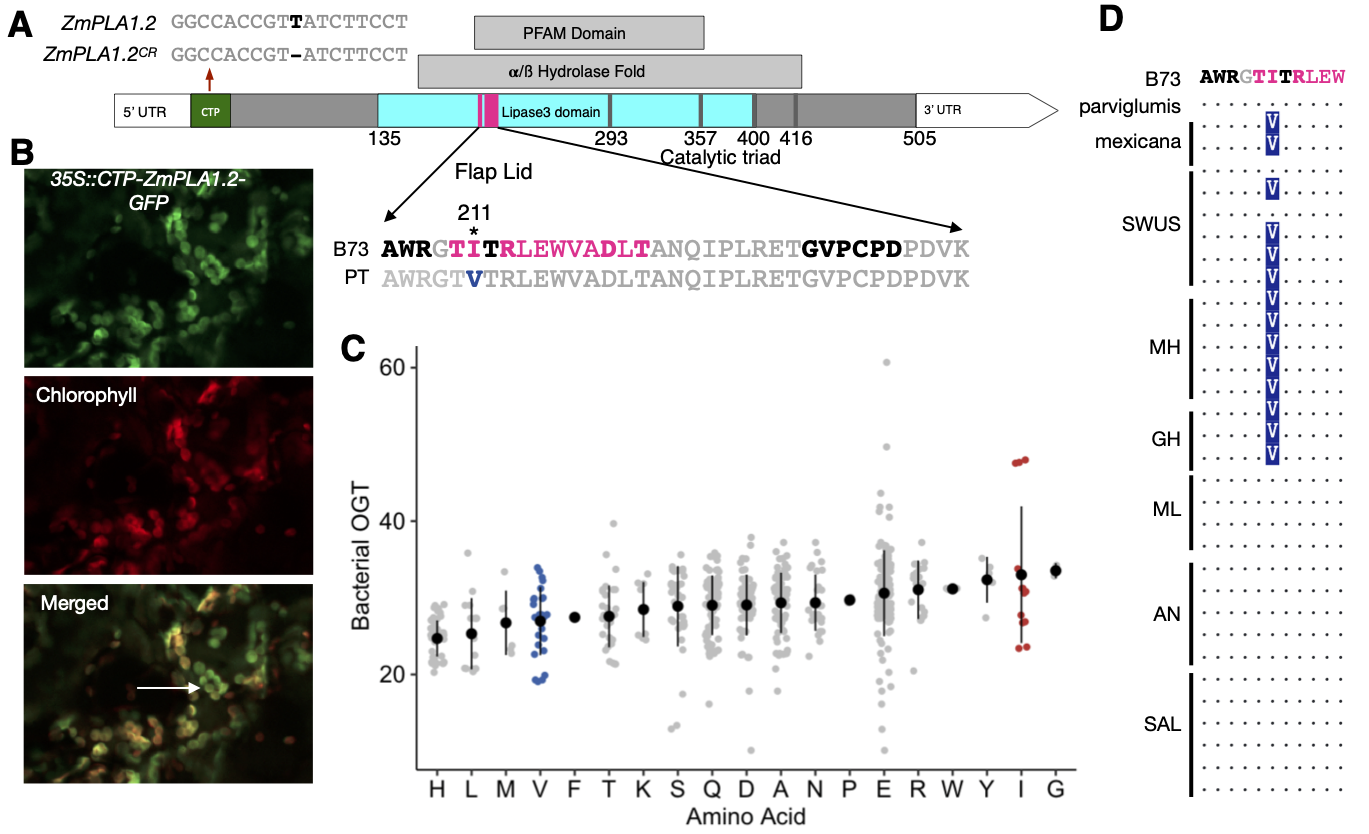
\includegraphics[width=0.8\paperwidth]{Figures/Fig_5.png}
\caption{\textbf{Fitness effects of the \textit{HPC1-PT} causal SNP and the \textit{hpc1\textsuperscript{CR}} mutant.} 
\textbf{A)} \textit{HPC1} coding sequence showing different features. 
CTP represents the chloroplast transit peptide. 
The arrow within CTP indicates the nucleotide insertion introduced by CRISPR/Cas9-mediated genome editing that leads to a frameshift.
Magenta indicates the coding sequence fragment that encodes the flap lid domain and the corresponding amino acids.
Residues in bold showed significant associations with prokaryote optimal growth temperature.
\textbf{B)} Prokaryote optimal growth temperature (OGT) test of different amino acids at the polymorphic residue 211 of HPC1.
\textbf{C)} Top I-TASSER model (plum) for the putative phospholipase encoded by HPC1-B73, overlaid on chain B of the crystal structure of phospholipase A1 from
Arabidopsis (PDB 2YIJ, tan). 
Residues that differ between the PT and B73 phospholipase are shown in yellow and some are labeled} 
\label{Fig5}
\end{center}
\end{figure*}

We then sought to identify candidate genes underlying the QTLs on chromosome 3.
The QTL contained 72 genes within its 1.5 LOD drop confidence interval (7.9-10 Mb) 
We hypothesized that the metabolic phenotypes we observed might be due to a gene involved in the process of PC-LPC conversion.  
The maize genome encodes 75 putative phospholipases (\ref{SupFig3}A), of which half are predicted to be phospholipase A1-type (PLA1) (\ref{SupFig3}A).  
We identified \textit{HPC1} (position on chromosome 3: 8,542,107 bp to 8,544,078 bp), within the QTL peak, as the most likely candidate (Figure \ref{Fig3}B). 
HPC1 has a predicted phospholipase A1-Igamma1 activity and can be classified, based on its two closest Arabidopsis orthologs (encoded by At1g06800 and At2g30550), as a PC-hydrolyzing PLA1 Class I phospholipase \cite{Ryu2004-iv}. 
PLA1-type phospholipases hydrolyze phospholipids in the sn-1 position and produce a lyso-phospholipid and a free fatty acid (\ref{SupFig3}B). 
Class I phospholipases are targeted to the chloroplast; indeed, we identified a chloroplast transit peptide (CTP) at the beginning of the predicted HPC1 sequence using the online tool ChloroP \cite{Emanuelsson1999-rs}.
We validated the chloroplast localization of HPC1 by transiently expressing  the HPC1 CTP fragment fused to green fluorescent protein (GFP) in \textit{Nicotiana benthamiana} leaves (\ref{SupFig4}).
In B73, \textit{HPC1} was one of the most highly expressed phospholipases, with expression almost exclusively restricted to vegetative leaves (V4-V9) (\ref{SupFig5}A) \cite{Stelpflug2016-vr}, which is the biological material we sampled for glycerolipid analysis. 
In B73 leaves, \textit{HPC1} was also the most highly expressed gene in the QTL interval (\ref{SupFig5}B \cite{Stelpflug2016-vr}).
%\textit{HPC1} is highly expressed in B73 and other temperate inbred lines under low temperature conditions and is downregulated in warm conditions (\ref{SupFig5}C) \cite{Waters2017-nat}.
%Note: we decided to not talk about this in the results. We do mention it in the discussion.
%Our results in the landrace diversity panel also  indicated that the PCs/LPCs levels were particularly high Mexican highland landraces. 
%We further studied PC, LPC selection using the individual species and individual PC/LPC species ratio. 
%The ratio of PC to LPC is higher in RILs that are homozygous PT at the \textit{HPC1} locus. 
%The differences are most stark in ratios where the LPC lipid species is presumably a product of the reaction, as the reaction is not occurring in PT lines. 
%For example, \textit{HPC1} would remove a 16:0 fatty acid from PC34:1 and leave LPC18:1 behind. 
%Our PBE, \textit{pcadapt}, $Q_{ST}$-$F_{ST}$ and QTL data strongly suggest that the PC-LPC balance is under selection in highland Mexican maize and that \textit{HPC1}, and to a minor extent, \textit{ZmLPCAT1} are themselves under selection and are major drivers of the lipid changes observed in highland maize. 
%Furthermore, the QTL data suggest that the highland PT allele is a impairedfunction of \textit{HPC1}. 

The effect of \textit{HPC1} on the PC/LPC levels may be caused by mis-regulation of \textit{HPC1} expression in highland landraces and/or by a mutation affecting the enzymatic activity of \textit{HPC1}. 
To distinguish between these two possibilities, we analyzed \textit{HPC1} expression in B73, PT and the corresponding F\textsubscript{1} hybrid plants grown at high or low temperatures to simulate highland and lowland conditions, respectively (Figure \ref{Fig3}E). 
Under cold conditions, \textit{HPC1-B73} was up-regulated, but \textit{HPC1-PT} was not (Figure \ref{Fig3}E). 
The lack of up-regulation in cold conditions of \textit{HPC1} may explain the high PC/LPC levels in PT.
However, the gene is expressed in PT at the same levels as in B73 under control conditions.
In the F\textsubscript{1} hybrids, \textit{HPC1} expression was consistent with a dominant B73 effect. 
We observed the same phenomenon for the PC/LPC ratio in the few B73 x PT BC1S5 RILs that are heterozygous at the \textit{HPC1} locus (\ref{SupFig3}C).
Variation in \textit{HPC1} may also (or in addition to any effects on expression levels) affect enzymatic activity of the HPC1-PT variant. In agreement with this notion, several PBE and \textit{pcadapt} outlier SNPs mapped to the \textit{HPC1} coding sequence rather than to regulatory regions. 
We used Sanger sequencing to analyze three B73 x PT RILs (B021, B042, B122) that are homozygous for the \textit{HPC1-PT} allele.
We discovered a recombination point 500 bp upstream of the \textit{HPC1} translation start codon (Figure \ref{Fig3}F, \ref{SupFig6}) in RIL B042, resulting in a chimeric gene with the coding region from PT, and a promoter segment from B73.
PC/LPC levels in RIL B042 were similar to other RILs that are homozygous for the PT haplotype at the 8.54 Mb marker at the QTL peak (Figure \ref{Fig3}F). 
This result supports the hypothesis that the metabolic effect we see is likely due to an impaired function of the HPC1-PT enzyme rather than to changes in the \textit{HPC1-PT} regulatory region.
If \textit{HPC1} is the underlying causal gene of this QTL, the observed metabolic phenotypes would be consistent with reduced or loss of function of the HPC1-PT enzyme leading to higher levels of PCs and lower levels of LPCs in the PT background. 
Next, we generated a genome-edited \textit{hpc1\textsuperscript{CR}} mutant via clustered regularly interspaced short palindromic repeats (CRISPR) and the CRISPR-associated nuclease Cas9 (Sup. File 4) in the B104 background, a temperate inbred derived from B73. 
We then measured PC and LPC species in wild-type and mutant plants grown under standard greenhouse conditions. 
\textit{hpc1\textsuperscript{CR}} plants recapitulated the effects seen for the \textit{PT} allele in the RILs (Figure \ref{Fig3} C-D bottom panels), further confirming that the \textit{HPC1-PT} allele impairs HPC1 function and thus underlies the QTL on chromosome 3 at around 8.5 Mb. 

Together, these data show that \textit{HPC1} underlies a major metabolic QTL explaining PC/LPC ratio. A mutation affecting the enzymatic activity of its encoded protein probably leads to impaired function in the highland PT allele.  

\subsection{\textit{HPC1} shows strong elevation-dependent antagonistic pleiotropy in Mexican landrace fitness phenotypes} 
We re-analyzed phenotypic data from a previously reported F1 association mapping panel \cite{Romero_Navarro2017-cn} \cite{Gates2019-xu}, by fitting a model to estimate the effect stemming from variation at \textit{HPC1-PT} on the relationship between fitness trait and elevation \cite{Runcie2019-Gr}. 
We determined that variation at \textit{HPC1} significantly affected G x E interactions for several fitness traits (Figure \ref{Fig4}). 
The effect of \textit{HPC1} on flowering time showed antagonistic pleiotropy between highland and lowland environments (Figure \ref{Fig4}). 
The highland \textit{HPC1-PT} allele was associated with delayed flowering in lowland environments (an increase of around one day in days to anthesis (DTA)  and 0.25 day for the  anthesis to silking interval (ASI)), but accelerated flowering at high elevation (with a decrease of DTA and ASI of one and 0.25 day, respectively) (Figure \ref{Fig4}).
Variation at \textit{HPC1} showed conditional neutrality on the fresh ear weight and grain weight per hectare traits: the highland allele had no effect in lowland environments, but was associated with greater values in highland environments (Figure \ref{Fig4}).

\subsection{Identification of the putative causal SNP in \textit{HPC1}.} 
We sequenced the \textit{HPC1} locus from several RILs harboring the PT haplotype at \textit{HPC1} and identified several of non-synonymous SNPs within the coding sequence that might influence HPC1 function (\ref{SupFig7})
We focused our attention on SNP 631 in the flap lid domain, which leads to a conservative replacement of isoleucine for valine (V211I, Figure \ref{Fig5}A).  
The flap lid domain is important for phospholipase activity and is located in a lipase class 3 domain (PFAM domain PF01764) that is highly conserved across the tree of life. 
We recovered 982 observations of the lipase class 3 PFAM domain from 719 prokaryotic species using PfamScan \cite{Potter2018-tk, El-Gebali2019-pw}, and estimated optimal growth temperatures from their tRNA sequences \cite{Cimen2020-dm}.
We then tested whether genetic variation in the lipase class 3 domain was significantly associated with optimal growth temperature in bacteria. 
We identified several significant associations, all of which were located in the flap lid region (Figure \ref{Fig5}B, bold letters).  
Notably, the presence of a valine at residue 211, as observed in the PT allele, was associated with lower bacterial optimal growth temperatures relative to bacterial lipases that harbor the isoleucine residue observed in B73 (Figure \ref{Fig5}B), suggesting that the PT allele may be better adapted to the low temperatures to which highland maize is exposed.
Figure \ref{Fig5} C shows the top I-TASSER model (plum) for the putative phospholipase encoded by \textit{HPC1-B73}, overlaid on chain B of the crystal structure of phospholipase A1 from Arabidopsis thaliana (PDB 2YIJ, tan). 
Residues that differ between the PT and B73 HPC1 are shown in yellow. 
The catalytic triad and H400 identified from CDD conservation analysis are also labeled.
However, our models put H416 in the catalytic triad instead of H400. 
Of the residues that differ between PT and B73 HPC1, residues 211, 448, and 449 are the closest to the catalytic triad. 
I211 is positioned on the N-terminal end of the flap lid domain and is well suited to stabilize, through hydrophobic interactions, binding of a lipid substrate.
Replacement of I211 with V211 results in the loss of a methyl group and may influence the strength of these hydrophobic interactions, influencing substrate binding and/or the dynamics of the flap lid domain.

\subsection{\textit{HPC1-PT} was introgressed from teosinte \textit{mexicana} and is conserved in Flint inbred lines} 
We next explored the segregation of the SNP causing the V211I change among other highland maize varieties.
We detected the PT allele at high frequencies in highland landraces from México and Guatemala. In addition, the PT allele segregated in Southwestern US landraces. 
The B73 allele was fixed in lowland Mexican, South American and Andean landraces (Figure \ref{Fig6}A). 
These results are consistent with our previous PBE results (Figure \ref{Fig2}E).
The PT allele was also present in teosinte, in one fourth of all teosinte \textit{parviglumis} accessions tested and in both \textit{mexicana} accessions reported in Hapmap 3 \cite{Bukowski2017-ng} (Figure \ref{Fig6}A). 
This observation prompted us to examine whether the PT allele was the result of post-domestication introgression from teosinte \textit{mexicana} during maize highland colonization, or whether it was selected from \textit{parviglumis} standing variation.

To test for introgression from \textit{mexicana}, we used \(f_d\) data from \cite{Gonzalez-Segovia2019-jy} and established that the genomic region containing \textit{HPC1} shows signatures of introgression from \textit{mexicana} into highland maize (Figure \ref{Fig6}B).
We then performed a haplotype network analysis using SNP data from the \textit{HPC1} coding region of 1,160 Mexican accessions from the SeeD Dataset \cite{Romero_Navarro2017-cn} that were homozygous for all SNPS across the coding region and the teosinte inbred lines (TIL) from Hapmap 3 \cite{Bukowski2017-ng}.   
We thus identified nine haplotype groups that cluster mainly based on elevation (Figure \ref{Fig6}C). 
The two major groups, II and VI, contained mainly lowland and highland landraces, respectively. 
The two \textit{mexicana} teosinte inbred lines (TIL08 and 25) belonged to group IV  (Figure \ref{Fig6}C) together with highland landraces primarily collected in the Trans-Mexican Volcanic Belt (30/36 from the highlands of Jalisco, Michoacán, México, Puebla and Veracruz).
We then examined whether this \textit{mexicana} haplotype (denoted \textit{ZxHPC1}) that is introgressed into Mesoamerican highland maize was also present in modern maize inbred lines. 
We performed a neighbor-joining cluster analysis using Hapmap 3 inbred lines including those from the 282 inbred panel, Teosinte inbred lines, German lines and PT. 
We identified two main groups, one containing the \textit{HPC1-PT} haplotype and the other containing the \textit{HPC1-B73} haplotype.
PT and the teosinte \textit{mexicana} inbred lines TIL-08 and TIL-25 clustered together with Northern European Flint inbred lines such as EP1, UH008, and UH009 (Figure \ref{Fig6}D). 
Other Northern US flints, e.g., CM7, are also closely related to the \textit{mexicana} \textit{ZxHPC1} haplotype. 
These data suggest that after introgression into highland maize, the \textit{ZxHPC1} haplotype was maintained in Flint materials adapted to cold environments in the Northern US, Canada and Europe. 

Building on previous reports for a role of highly unsaturated PC species in determining flowering time \cite{Nakamura2014-qf, Riedelsheimer2013-bd} and considering the significant accumulation of those PC species induced by the \textit{HPC1-PT} allele, we asked if variation in \textit{HPC1} might be associated with differences in flowering time in modern maize. 
We used a large gene expression dataset obtained from the 282 maize diversity panel that was sampled across several developmental stages \cite{Kremling2018-gn}, and phenotypic datasets collected from the same panel grown in long days and short days.
We discovered that \textit{HPC1} and \textit{ZmLPCAT1} expression levels are inversely correlated in most tissues (\ref{SupFig8}), further supporting the idea that these two enzymes are coordinately regulated. 
There were significant associations between \textit{HPC1} expression levels in aerial tissues and several flowering time traits.
The magnitude of these associations was similar to those seen for other well-characterized flowering time genes (\ref{SupFig8}) such as \textit{ZEA CENTRORADIALIS8} (\textit{ZmZCN8})  and the AP2/ERF transcription factor gene \textit{ZmRAP2.7}.  
Furthermore, in both long days and short days, lines carrying the \textit{HPC1-PT} allele were characterized by lower \textit{HPC1} expression and earlier flowering times relative to lines carrying the \textit{HPC1-B73} allele (Figure \ref{Fig6}E). 

Taken together, these data show that \textit{HPC1} was introgressed from teosinte \textit{mexicana} into highland maize and that this introgression was carried over into high latitude adapted modern inbred lines that show low \textit{HPC1} expression in association with early flowering.

 \section{Discussion}
\label{sec:discussion}
Understanding the genetic, molecular and  physiological basis of crop adaptation to different environments and the role that wild relatives have played in these processes is relevant for the identification of favorable genetic variation that can be used to improve modern crops.
The repeated events of maize adaptation to highland environments constitute an excellent natural experiment to study crop local adaptation. 
Recent studies \cite{Wang2020-mp, Takuno2015-uj, Crow2020-gene} have helped expand our understanding of the genetic basis underlying maize highland adaptation. However, the molecular, physiological and genetic mechanisms underlying maize highland adaptation and the possible role of highland maize traits in modern, commercial varieties remain largely unknown.
Phospholipids are key structural components of plant membranes that also function as signaling molecules during adaptation to stresses that would be prevalent in highland environments \cite{Ryu2004-iv, Nakamura2017-vb} such as low phosphorus availability \cite{Veneklaas2012-ls, Cruz-Ramirez2004-ib, Lambers2012-an} and low temperatures \cite{Degenkolbe2012-wf, Welti2002-uk, Marla2017-ph}. 
Additionally, in Arabidopsis, accumulation of certain highly unsaturated PC species can accelerate flowering time \cite{Nakamura2014-qf}, which is a major driver of maize adaptation to highland environments \cite{Romero_Navarro2017-cn, Gates2019-xu, Mercer2019-vj}.

\begin{figure*}[!ht]
\begin{center}
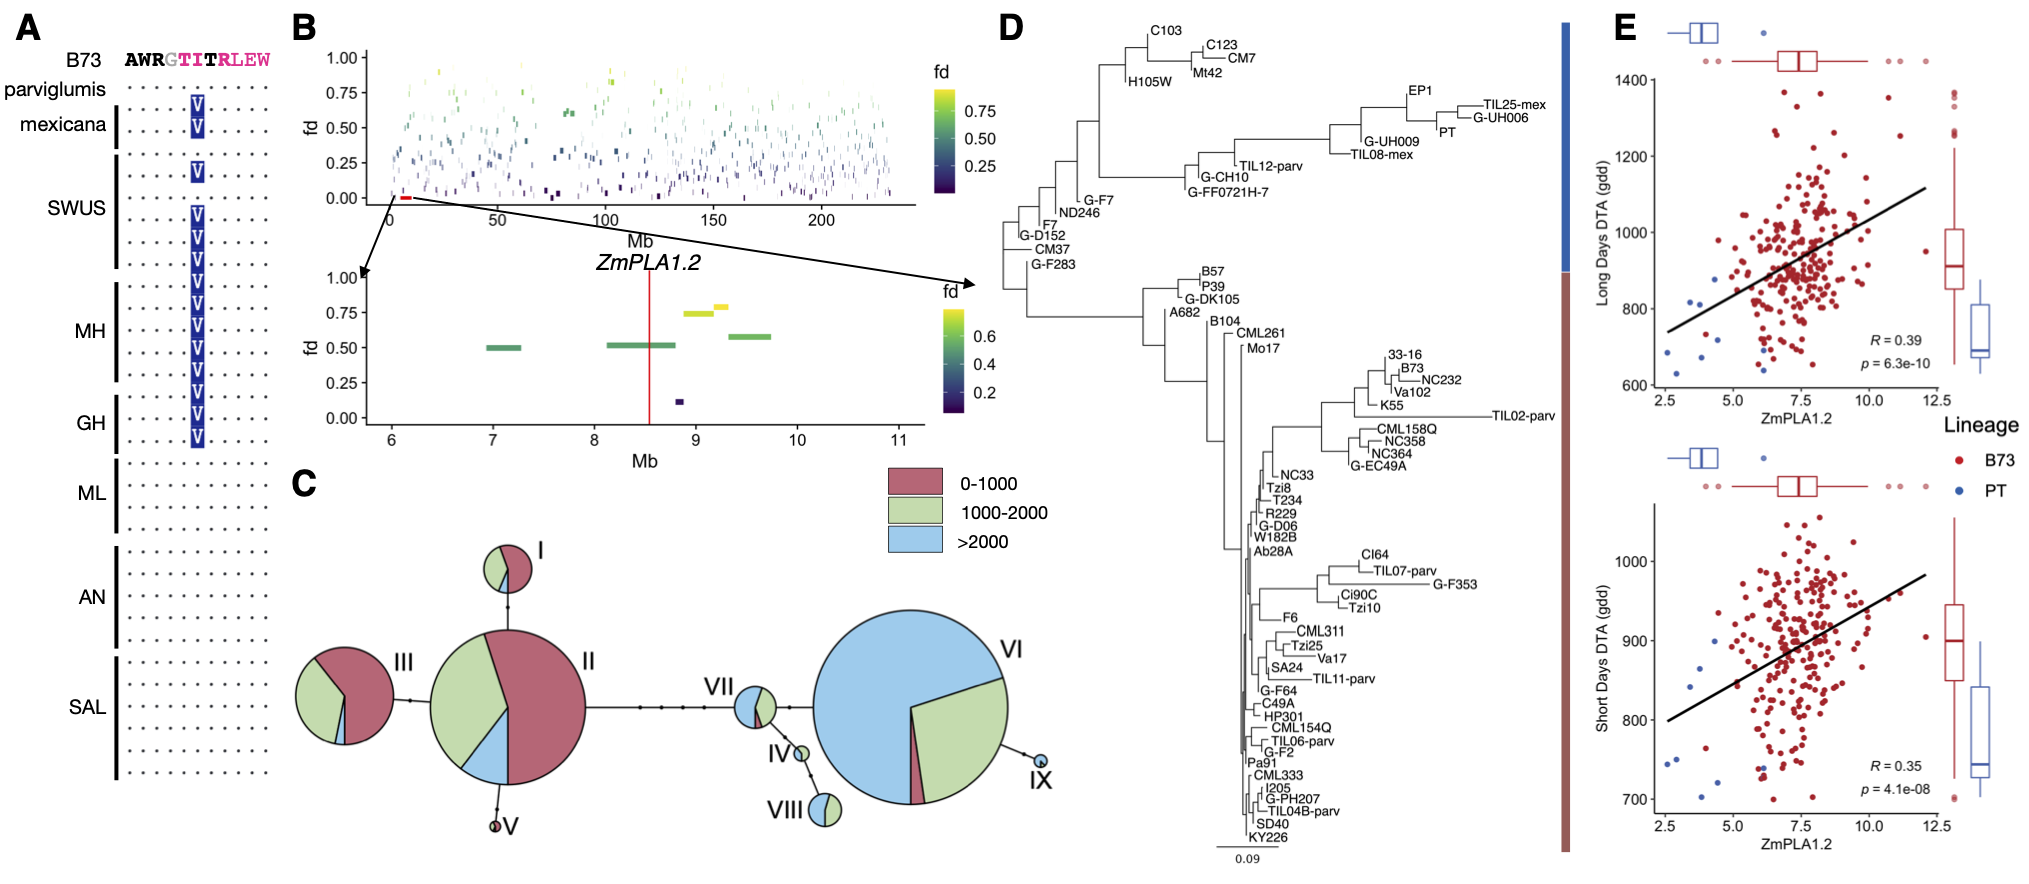
\includegraphics[width=0.8\paperwidth]{Figures/Fig_6.png}
\caption{\textbf{Introgression of teosinte \textit{mexicana} into maize \textit{HPC1}.}  
\textbf{A)} Alignments around the V211I polymorphism in the flap-lid domain of HPC1 in B73, \textit{mexicana} and \textit{parviglumis} and landraces of the Southwestern US (SWUS), Mexican Highland (MH) and Lowlands (ML), Guatemalan Highlands (GH), Andes (AN) and South America Lowlands (SAL).
\textbf{B)} \(f_d\) analysis of the \textit{mexicana} introgression. Data were obtained from \cite{Gonzalez-Segovia2019-jy}. 
\textbf{C)} Haplotype network analysis of SNPs within the \textit{HPC1} coding region, using 1,060 Mexican homozygous individuals from the SeeD dataset.
\textbf{D)} Cluster analysis of the \textit{HPC1} coding region using a sample of Hapmap3 inbred lines and the PT landrace.
\textbf{E)} Correlation between \textit{HPC1-PT} expression and days to anthesis (DTA) in plants grown in short or long days. 
Inbred lines from the PT lineage shown in panel C are indicated in blue and inbred lines from the B73 lineage are in red;
data from \cite{Kremling2018-gn}.}
\label{Fig6}
\end{center}
\end{figure*}
 
We used genomic scans and linkage mapping analysis to identify and clone \textit{High PhosphatidylCholine 1} (\textit{HPC1}), which encodes a phospholipase A1 enzyme with a major role in determining phosphatidylcholine levels in highland maize landraces.
We described how genetic variation at this locus shows strong antagonist pleiotropic G X E effects on several fitness traits.
We then showed that the highland allele is the result of an introgression from teosinte \textit{mexicana} that has been maintained in modern maize inbred lines adapted to high latitudes.
%that genes involved in the synthesis and degradation of PC species, such as \textit{HPC1} and \textit{ZmLPCAT1}, have been repeatedly selected in maize highland populations, leading to high PC/LPC ratios.   
%We then identified \textit{HPC1} as the gene underlying a major effect PC/LPC QTL in a B73 x Palomero Toluqueño RIL population. 
%The effect of the highland PT allele indicates it is impaired in function, possibly due to single point mutation in the flap-lid domain that reduces the efficiency of PC to LPC conversion. 
%The impact of genetic variation at \textit{HPC1} showed strong GxE effect with respect to elevation, delaying flowering in lowland environments but  accelerating flowering in highlands (Fig. \ref{Fig4}A).
%This effect was further confirmed in the CRISPR-CAS9 missense mutant, \textit{HPC1\textsuperscript{CR}}.
%We then found that the highland \textit{HPC1} haplotype is the result of teosinte \textit{mexicana} introgression that is still conserved in Northern USA, Canada and EU Flints. 
%Sequencing of the \textit{HPC1-PT} allele identified a SNP in the flap lid domain of the phospholipase that may probably affect substrate specificity and enzymatic activity.
%Indeed, a CRISPR KO mutant of \textit{HPC1} phenocopied the highland \textit{HPC1-PT} allele. 
%Evaluation of protein residue variation of the PFAM domain across hundreds of bacteria species further confirmed that the protein residue variation in the flap lid domain is associated with bacterial optimal growth temperature.
%We then found that the \textit{HPC1-PT} is conserved in Mexican and Guatemalan highland maize and to a lesser extent in Southwestern US maize and that this highland allele is the result of highland teosinte \textit{mexicana} into highland maize. 
%Moreover, the  \textit{ZxHPC1.2/HPC1-PT} haplotype is conserved in Northern US and European Flints and that lower expression of \textit{HPC1} is low in this Flint material and is correlated with faster flowering times.
%Finally, using phenotypic and genotypic data of thousands of Mexican accessions grown in several common garden trials across Mexico we show that genetic variation of \textit{HPC1} shows a strong G x E interaction where the highland allele leads to a delay of flowering time in lowland environments and an acceleration of flowering time in highland environments. 
%Other fitness related phenotypes show a similar G X E interaction where the highland \textit{HPC1} leads to more fit plants in highland environments and less fit plants in lowland environments. 
%This effect was confirmed using a CRISPR mutant of \textit{HPC1}.
%Our data indicate that \textit{HPC1} is a major component of the phpospholipid makepup of maize that can influence several fitness phenotypes important in maize adaptation to low temperatures through physiological and molecular mechanisms that will need to be further investigated.
%Given the important role of this environmental factors and plant traits in highland environments, we hypothesized that phospholipid metabolism has been important in the repeated events of maize highland adaptation. 
%We studied selection of pathways involved in glycerolipid metabolism (that includes phospholipids but also other non-phosphorus containing polar lipids such as galactolipids) at the genetic pathway level using a Population Branch Excess approach \cite{Pool2017-oa, Wang2020-mp}. 

Genes involved in the biosynthesis and degradation of phospholipids were repeatedly selected in several highland maize populations of North America, Central America and South America (Figures \ref{Fig1} and \ref{Fig2}). 

\textit{ZmLPCAT1} and \textit{HPC1} were two of the genes that showed the strongest, repeated signals of selection, as measured by PBE and \textit{pcadapt} in highland populations (Figure \ref{Fig2}). 
In a previous study, \textit{ZmLPCAT1} exhibited high \textit{Fst} values when highland and lowland landraces were compared \cite{Takuno2015-uj}.
The predicted function of ZmLPCAT1 is to synthesize PC species via the acylation of LPC species, while HPC1 is predicted to hydrolyze PCs into LPCs and free fatty acids by cleaving the sn1-position.
Selection at these two loci is likely to have driven the high PC/LPC ratio we observed in highland Mexican landraces (Figure \ref{Fig1}).
Natural variation at maize \textit{HPC1} is associated with lipid levels \cite{Riedelsheimer2012-bx} and flowering time \cite{Chen2012-gg, Hung2012-ms}. 
In B73, \textit{HPC1} is one of the most highly expressed phospholipase-encoding genes and its expression pattern is almost entirely restricted to vegetative leaves (V4-V9) (\ref{SupFig3}C) \cite{Stelpflug2016-vr}, which we sampled for our glycerolipid analysis. 
In B73 leaves, \textit{HPC1} is the most highly expressed gene within  the QTL interval (7.9 Mb to 10 Mb) (\ref{SupFig5}B \cite{Stelpflug2016-vr}).
In addition, \textit{HPC1} is highly expressed in B73 and other temperate inbred lines grown in low temperature conditions and is down-regulated by heat stress (\ref{SupFig3}D) \cite{Waters2017-nat}.
In our experiments, \textit{HPC1} was up-regulated in B73 and the B73 x PT F\textsubscript{1} hybrids after cold exposure. 
By contrast, the \textit{HPC1-PT} allele was expressed at similar levels as \textit{HPC1-B73} in control conditions, and was not up-regulated in cold conditions (Figure \ref{Fig3}E).
In Arabidopsis, \textit{LPCAT1} is involved in modulating phosphorus levels in leaves under low zinc conditions \cite{Kisko2018-zm}.
In maize, a positive signal from a genome-wide association study (GWAS) 45 kb upstream of \textit{ZmLPCAT1} was associated with flowering time under low phosphorus conditions, further lending support to a possible role for natural variation at \textit{ZmLPCAT1} in plant adaptation to low phosphorus availability. 

Our QTL analysis of the PC/LPC ratios in a B73 x PT mapping population and in the \textit{hpc1\textsuperscript{CR}} mutant demonstrates that the highland \textit{HPC1-PT} allele results in an enzyme with impaired function that alters highland Mexican maize PC metabolism, leading to higher PC/LPC ratios (Figure \ref{Fig3}). 
Using the PC/LPC ratio as a phenotype, we obtained much more significant LOD QTL signals than when using PC or LPC levels alone, possibly because the ratio can much more precisely capture genetically-induced changes in enzymatic activity \cite{Petersen2012-ii}.
Adaptive loss-of-function mutations can be an effective way to gain new metabolic functions in new environmental conditions \cite{Hottes2013-np}. 
Our data illustrate how an enzymatically impaired enzyme, due to a single conservative amino acid replacement located in the flap lid domain of HPC1,  can affect substrate  accessibility and/or substrate binding (Figure \ref{Fig5}A). 
Indeed, the flap lid domain has been the target of biotechnological modification of these types of enzymes \cite{Khan2017-ua}.

Why were the metabolic changes induced by HPC1 variation selected for in highland maize?
PC metabolism is intimately connected to multiple stress responses and developmental pathways; alterations in PC amounts and PC/LPC ratios affect overall plant fitness.
The \textit{qPC/LPC3@8.5} QTL is driven by individual QTLs of PC and LPC species with high levels of unsaturated fatty acids (\ref{SupFig2}).
Several of these species, like PC 36:5 and LPC 18:1 (Figure \ref{Fig3}D, Sup. File 3), have been shown to display similar patterns during Arabidopsis cold acclimation \cite{Welti2002-uk} and sorghum (\textit{Sorghum bicolor}) low temperature responses \cite{Marla2017-ph}.
PC 36:5 also showed high $Q_{ST}$ values when comparing highland and lowland landraces from both Mesoamerica and South America (Figure \ref{Fig1}C-D, Sup. File 5).
In maize, \textit{HPC1} expression is under the control of the circadian clock \cite{Khan2010-iv} with a peak at the end of the day. 
In Arabidopsis, highly unsaturated PC (34:3, 34:4, 36:5, 36:6) species increase in the dark \cite{Maatta2012-ip}. 
This peak of concentration coincides in maize with low expression levels of \textit{HPC1} during the same dark hours \cite{Khan2010-iv}.
Furthermore, Yuki Nakamura and colleagues elegantly demonstrated that PC 36:5 and 36:6 species accumulate during the night and can bind to Arabidopsis FLOWERING LOCUS T (FT) to hasten flowering \cite{Nakamura2014-qf} by unknown cellular mechanisms. 
The Arabidopsis \textit{FT} ortholog in maize, \textit{ZCN8} \cite{Lazakis2011-nq}, underlies a major flowering time and photoperiod sensitivity QTL \cite{Hung2012-ms}.
Additive mutations in the regulatory region of \textit{ZCN8}, including a teosinte \textit{mexicana} introgression, lead to higher expression of \textit{ZCN8}, which contributes to maize adaptation to long days in temperate conditions \cite{Guo2019-pn}.
Our results show that HPC1 drives the accumulation of the same PC species (such as PC 36:5) that accumulate in Arabidopsis at the end of the day, at which time they might bind to FT and activate the transition from vegetative to reproductive development. 
We hypothesize that the accumulation of these PC species in highland maize may drive early flowering in a manner similar to that in Arabidopsis. 

The effects of genetic variation at \textit{HPC1} on flowering time in Mexican landraces indicated a strong GxE interaction, whereby the highland allele leads to an acceleration of flowering and ASI in highland environments (Figure \ref{Fig4}), similar to the effects observed with the well-known teosinte \textit{mexicana} introgression \textit{inv4m} \cite{Crow2020-gene}.
Other flowering time loci analyzed did not show this clear G x E effect \cite{Gates2019-xu}.
Interestingly, the effect of the highland allele exhibited typical conditional neutrality in yield-related traits, with increased fitness conferred by the \textit{HPC1-PT} allele in highlands (Figure \ref{Fig4}).

The mutation in the flap-lid of HPC1-PT at residue 211 is conserved in highland Mexican and Guatemalan landraces and in teosinte \textit{mexicana} (Figure \ref{Fig6}A) but is still segregating in teosinte \textit{parviglumis}. 
We showed that \textit{HPC1-PT} is  indeed an introgression from teosinte \textit{mexicana} (Figure \ref{Fig6}B) and that this introgression has been maintained in modern inbred lines, particularly in the Northern US, Canadian and European Flint lines (Figure \ref{Fig6}D). 
\textit{HPC1} in inbred lines carrying the \textit{ZxHPC1} \textit{mexicana} haplotype was expressed at low levels and resulted in earlier flowering (Figure \ref{Fig6}E) \cite{Kremling2018-gn}. 
Other grasses such as eastern gamagrass (\textit{Tripsacum dactyloides}) are adapted to temperate latitudes and also show accelerated rates of evolution in genes involved in PC metabolism \cite{Yan2019-tx}.
Moreover, genetic variation in the regulatory region of \textit{HPC1} was significantly associated with photoperiod sensitivity in the maize Nested Association Mapping population \cite{Hung2012-ms}. 

In summary, we used here a combination of genomic scans, linkage mapping, lipidomics and reverse genetics to identify and clone the adaptive gene \textit{HPC1}, introgressed from teosinte  \textit{mexicana}, in highland maize landraces. HPC1 leads to a major reorganization of phosphatidylcholine metabolism. 
We showed that the fitness advantage conferred by the \textit{HPC1} highland \textit{mexicana} allele is at least in part due to its effect on accelerating flowering and that this effect may have contributed to adaptation of maize to cold, high latitudes. 
This study highlights the largely underappreciated role of highland maize and highland teosinte \textit{mexicana} in modern maize.

\section{Materials and Methods}
\label{sec:materials:methods}
\textbf{Populations used in the analysis.} 
Highland and lowland populations used for Population Branch Excess analysis consisted of three to six accessions from each of the highland and lowland populations and have been previously described in \cite{Wang2020-mp, Wang2017-bc}. 
The 120 landraces from the HiLo diversity panel were selected and ordered from the \href{http://mgb.cimmyt.org/gringlobal/search.aspx}{CIMMYT germplasm bank} to maximize a good latitudinal gradient sampling across Mesoamerica and South America. 
For each highland landrace (>2,000 meters above sea level [masl]) a lowland landrace (<1,000 masl) was selected at the same latitude (<0.5\degree) to form 60 highland/lowland pairs, with 30 from each continent. 
The list of the accessions used is provided in Sup. file 1.   
B73 x Palomero Toluqueño (PT) recombinant inbred lines (RILs) were developed by crossing B73 with a single PT plant (Mexi5 accession, CIMMYTMA 2233) that was then backcrossed with B73 once and selfed five times (BC1S5).  
We used  individual landrace accession genotype and fitness data from the CIMMYT Seeds of Discovery project (SeeD) \cite{Gates2019-xu} to calculate \textit{pcadapt} \cite{Luu2017-ws} values and GxE effects of \textit{HPC1-PT}.

\textbf{Field Experimental Conditions and sampling.} 
Two replicates of the HiLo diversity panel accessions and three replicates of the B73 x PT RILs were planted in a highland and lowland common gardens. 
The highland common garden was located in Metepec, Edo de México, (19\degree13'28.7"N 99\degree32'51.6"W) in the Trans-Mexican volcanic belt. 
The field is at 2,610 masl, and the range of average monthly temperatures along the year vary from 5\degree C to 21.5\degree C.  
The lowland common garden was located in Valle de Banderas, Nayarit, (20\degree47'01.2"N 105\degree14'47.0"W) in the Pacific Coast. 
The field is at 50 masl, and the range of average monthly temperatures along the year vary from 20\degree C to 29\degree C.
Between growth stages V4 and V6, we used a leaf puncher to collect 50 mg of fresh tissue (10 discs) from the tip of the second leaf above the last leaf with a fully developed collar. 
Tissue discs were immediately flash-frozen in liquid nitrogen. 
We collected all samples from a field in a single day between 10:00 am and 12:00 pm, approximately 3 h after sunrise.
Samples were transported in dry ice to the lab and stored at --80\degree C until extraction. 

\textbf{Glycerolipid analysis} 
We crushed frozen samples in a Retsch tissue grinder (Haan, Germany) for 40 seconds at a frequency of 30 pulses per second. 
We performed lipid extraction following Matyash and collaborators \cite{Matyash2008-ue}. 
First, we added 225 $\upmu$L of cold methanol (MeOH) to each sample. 
For the blanks, we prepared MeOH containing a Quality Control (QC) mix (Sup. File 6).
We vortexed each sample for 10 sec, keeping the rest of the material on ice. 
Then, we added 750 $\upmu$L of cold methyl tert-butyl ether (MTBE). 
For the blanks, we used MTBE containing 22:1 cholesterol ester as internal standard (Sup. File 6). 
We vortexed each sample for 10 sec, followed by 6 min of shaking at 4\degree C in the orbital mixer. 
We next added 188 $\upmu$L of LC/MS grade water at room temperature (RT), and vortexed samples for 20 sec.
We centrifuged the samples for 2 min at 14,000 rcf and recovered 700 $\upmu$L of supernatant from the upper organic phase. 
We then split the supernatant into two aliquots of 350 $\upmu$L each, one aliquot was used for the generation of the lipid profile and the other aliquot was used to prepare pools that were used along the lipid profiling. 
Finally, we dried the samples using a speed vacuum concentration system.
We resuspended dried samples in 110 $\upmu$L of MeOH-Toluene 90:10 (with the internal standard CUDA, 50 ng/mL). 
We vortexed samples at low speed for 20 sec and then sonicated them at RT for 5 min. 
We then transferred aliquots of 50 $\upmu$L per sample into an insert within an amber glass vial.
The UHPLC-QTOF MS/MS utilized were Agilent 1290 and Agilent 6530, respectively. 
We used a Waters Acquity charged surface hybrid (CSH) C18 2.1x100 mm 1.7 $\upmu$m column which we initially purged for 5 min. 
We coupled the UHPLC column with a VanGuard pre-column (Waters Acquity CSH C18 1.7$\upmu$m). 
We injected six “no sample injections” at the beginning of each run to condition the column, followed by ten samples, one pool (made out of the mix of the second aliquot of all the samples contained per UHPLC plate) and one blank.
We injected 1.67 $\upmu$L per sample into UHPLC-QTOF MS/MS ESI (+); the running time per sample was 15 min. 
Mobile phase “A” consisted of 60:40 acetonitrile:water, 10 mM of ammonium formate and 0.1\% formic acid. 
Mobile phase “B” consisted of 90:10 isopropanol:acetonitrile, 10 mM ammonium formate and 0.1\% of formic acid. 
The flow rate was 0.6 mL/min and the column compartment was maintained at 65° C. Initial conditions were 15\% B; the gradient uniformly increased until reaching 100\%. 
At 12.10 min the mobile phase composition returned to initial conditions.
We used the mass spectrometer (Q-TOF MS/MS) in positive electrospray ionization mode (ESI).
The source parameters were: ESI gas temperature 325 \degree C, nebulizer pressure 35 psig, gas flow 11L/min, capillary voltage 3500 V, nozzle voltage 1000 V, and MS TOF fragmentor and skimmer 120 and 65 V, respectively.
We used a mass range between 60 and 1,700 m/z, under acquisition parameters. 
As for reference mass parameters, we used a detection window of 100 ppm and a minimum height of 1,000 counts. 
We performed a retention time (rt) correction of the acquired data using Agilent MassHunter Qualitative Analysis B.06.00 version and Microsoft Excel. 
To extract ion chromatograms (EICs) of the internal standards within the run we used Agilent MassHunter Qualitative Analysis.
We identified the time of the highest intensity point of each EIC, which we used as the current retention time of the experiment. 
We used the method retention time for internal standards and the current rt and we fitted a polynomial regression to calculate new retention times using retention times from 501 lipids of a MS1 m/z-rt library (See Sup. File 7). 
In MSDIAL \cite{Tsugawa2015-kh}, identification of lipids is based on two approaches: the MSP file and MS/MS identification setting included in MSDIAL and the use of a post identification file containing accurate m/z and rt for a list of lipids. 
In this study we used both identification approaches. 
Under positive ion mode, the MSP file and MS/MS identification setting has a total of 51 lipid classes  selectable for identification. 
The post identification file that we used was the retention time-corrected MS1-MS2 mz-rt lipid library that we explained before. 
We used MSDIAL \cite{Tsugawa2015-kh} version 3.40. 
To use MSDIAL, we converted the raw data from .d to .abf format with Reifycs Abf converter (https://www.reifycs.com/AbfConverter/). 
Then, we filtered the MSDIAL alignment results based on whether compounds intensity was ten times above blank intensity. Next, filtered data were normalized using Systematic Error Removal using Random Forest (SERRF) \cite{Fan2019}. This normalization is based on the QC pool samples. 
We filtered out, now the normalized features, considering a coefficient of variation (CV) equal or less than 30\% among the pools. 
To curate the data for duplicate features, isotopes and ion-adducts, we utilized MS-FLO \cite{DeFelice2017-ms}.
We also normalized the curated data using the sum of all known metabolite signal (mTIC). 
After data processing and normalization, we used lipid intensities for further analysis.

\textbf{CRISPR-CAS9 Glycerolipid analysis}
Dry samples were resuspended in 110 $\upmu$L of 100\% MeOH (with the internal standard CUDA, 50 ng/mL), vortexed at low speed for 20 s and then sonicated at RT for 5 min. 
We transferred the samples into amber glass vials with inserts prior to analysis. 
Lipid profiling was performed using a Thermo Scientific Orbitrap Exploris 480 mass spectrometer coupled to a Thermo Vanquish Horizon UHPLC. 
Chromatographic separation was achieved using the same guard and analytical column type, mobile phase composition and gradient conditions described for UHPLC-QTOF analyses. 
Avanti Splash Lipidomix Mass Spec Standard (Avanti Polar Lipids, Alabaster, Alabama) was used to check system suitability and a Lipid QC Standard Mixture (Sup. File 6) and pooled QC samples were used to monitor instrument performance. 
Methanol solvent blanks were injected at the beginning of the sequence and throughout the batch between approximately 10 injections and pooled QC samples were injected between every 6–8 sample injections. 
For ion source parameters the spray voltage was set at 3500 V, sheath gas 60 (arb), aux gas 15 (arb), sweep gas 2 (arb) and ion transfer tube and vaporizer temp at 350 \degree C. 
Full scan and data-dependent MS/MS (ddMS\textsuperscript{2}) scans were collected in positive ESI mode following 2 $\mu$L sample injections. 
Full scan spectra were obtained from \textit{m/z} 220--1700 using an Orbitrap resolution setting of 120,000, RF lens set at 25\%, normalized AGC target at 25\% and maximum injection time set to auto. 
ddMS\textsuperscript{2} scans were performed using a cycle time of 0.6 sec, intensity threshold of 5.0e4, and a 3 sec dynamic exclusion using a 10 ppm mass tolerance. 
Additional parameters for ddMS\textsuperscript{2} experiments were as follows: Isolation window equal to 1 Da, stepped collision energy at 20 and 30\%, Orbitrap resolution set to 15,000, scan range set to auto, normalized AGC target of 100\% and a maximum ion injection time of 55 msec. 
Data files were uploaded to LipidSearch 4.2.2 (Thermo Scientific, Tokyo, Japan) for identification of PC and LPC species. 
Skyline-daily \cite{Adams2020-em} was then used to obtain normalized peak areas for the identified PCs and LPCs using the internal standards PC(12:0/13:0) and LPC(17:0), respectively.

\textbf{$\mathbf{Q_{ST}-F_{ST}}$ analysis of glycerolipid data.}
Quantitative trait differentiation ($Q_{ST}$) was contrasted to the distribution of $F_{ST}$ for neutral genetic markers \cite{whitlock2008evolutionary}.
Highland/Lowland contrasts were considered separately for Mesoamerica and South America.
A linear mixed effects model (R package lmer, function lmer) was used to partition phenotypic variance between population pairs (Mesoamerica/South America, all highland/all lowland, Mesoamerican highland/Mesoamerican lowland, South American highland/South American lowland).
\begin{center}
${ TRAIT \sim 1 + (1|POPULATION) + }$\\
${(1|GARDEN/BLOCK) + (1|BATCH)}$
\end{center}
Within-population and between-population variances were calculated with the R function VarCorr (R package \texttt{lme4}, \citealp{bates2014lme4}), and were used to calculate $Q_{ST}$ following the equation below:
\begin{center}
$Q_{ST}$ = \(\sigma^{2}_{GB}/(\sigma^{2}_{GB}+2\sigma^{2}_{GW})\)
\end{center}
\noindent in which $\sigma^{2}_{GB}$ and $\sigma^{2}_{GB}$ are the between- and within-population genetic variance components, respectively \cite{Leinonen2013-ic}.
Pairwise $F_{ST}$ was calculated with the R function fst.each.snp.hudson (R package \textit{dartR}, \citealp{gruber2018dartr}).

\textbf{\textit{pcadapt} analysis of biological adaptation in Mexican landraces.}
In order to conduct genome scans for signatures of adaptation we used the \textit{pcadapt} \cite{Luu2017-ws} package.
\textit{pcadapt} identifies adaptive loci by measuring how strongly loci are contributing to patterns of differentiation between major axes of genetic variation.
Under simple models \textit{pcadapt} captures major patterns of $F_{ST}$  but is conducted in a way that does not require population delimitation \cite{duforet2014genome}.
As the genome scan comparison requires a focal SNP to be compared to the first K principal components of the genotype data, it can be biased by large regions of low recombination that drive the major axes of variation in the principal components.
Thus, when SNPs from these low recombination regions are compared against principal components driven by linked loci spurious signals may arise.
To prevent this bias from occurring, we used custom scripts to calculate the principal component step separately based upon all the chromosomes except for the chromosome of the focal SNPs being tested.
The genotype data we used for this analysis was GBS data from roughly 2,000 landraces of Mexican origin collected by CIMMYT (www.cimmyt.org) as part of the SeeDs of discovery initiative (https://www.cimmyt.org/projects/seeds-of-discovery-seed/).
From this, we calculated the strength of association between each SNP and the first five principal components (excluding the chromosome of the focal SNP) using the communality statistic as implemented in \textit{pcadapt} version 3.0.4.

\textbf{Glycerolipid pathways selection.}
We compiled a list of genes pertinent to glycerolipid metabolism starting with a search of all genes belonging to the \textit{Zea mays} 'Glycerophospholipid metabolism' and 'Glycerolipid metabolism' KEGG pathways \cite{kanehisa2019} (map identifiers: zma00564 and zma00561). 
With the NCBI Entrez gene identifiers in KEGG we retrieved the AGPv4 transcript identifiers used in Corncyc 8.0 \cite{portwood2019, walsh2016} from an id cross reference \href{https://www.maizegdb.org/search/gene/download_gene_xrefs.php?relative=v4}{file} found in MaizeGDB   \cite{portwood2019}.
This resulted in a list of 300 genes comprising 51 Corncyc pathways. 
Then we discarded Corncyc pathways  tangentially connected to the KEGG glycerolipid metabolism list (sharing just one enzyme with the initial KEGG list) or that we judged to belong to different biological processes (e.g 'long chain fatty acid synthesis','anthocyanin biosynthesis'). 
Finally, we added manually the 'phosphatidylcholine biosynthesis V' pathway that was missing. 
The list of 30 selected Corncyc pathways included genes outside the initial KEGG search results and raised the number of genes to 557. 
In addition to these, 37 genes were found to have an enzymatic activity related to phospholipid metabolism but not placed into any particular pathway, i.e orphan enzymes, consisting mostly of alcohol dehydrogenases. 
Sixteen additional genes found in KEGG were not annotated at all in Corncyc probably due to differences between AGPv4 and RefSeq pseudogene annotation of the maize genome. 
The list of all possible candidates coming either from KEGG or Corncyc that were orphan enzymes or were unannotated in Corncyc amounted to 594 genes (Sup. File 2). 
This process is documented in the \verb|0_get_glycerolipid_genes.R| script of the \verb|pgplipid| R package accompanying this paper \cite{fausto_rodriguez_zapata_2020_4323410}.

\textbf{Population Branch Excess Analysis.}
Population Branch Excess quantifies changes in allele frequencies in focal populations relative to two independent “outgroup” populations.
We used \textit{Zea mays spp. parviglumis} as one of the outgroup populations for all four highland groups.  
The other outgroup was  Mexican lowlands  in the case of Southwestern US , Mexican highlands and Guatemalan highlands; and South American lowlands in the case of the Andes population. 
We used calculated PBE SNP values for the four populations (described in detail in \cite{Wang2020-mp}) and we tested for selection outliers SNPs in the 594 phosphoglycerolipid-related candidate genes and the 30 Corncyc pathways (556 genes).
We first defined PBE outlier SNPs as the top 5\% of the PBE score distribution; this fraction corresponds to approximately 50000 out of ~1 million genotyped SNPs in each population. 
Following \cite{Wang2020-mp}, we defined a gene as a PBE outlier if it contained an outlier SNP within the coding sequence or 10 kb upstream/downstream. 
Then we tested for over-representation of genes selected in particular subsets of populations using Fisher's exact test with the 32,283 protein-coding genes from the maize genome as background. 
For each pathway, we first selected all SNPs within coding regions and 10 kb upstream and downstream of genes in the pathway and we calculated the mean pathway PBE score. 
We then constructed a null distribution by drawing 10,000 samples without replacement of $n$ SNPs from those found within or around 10 kb upstream and downstream of all protein-coding genes and we obtained the mean PBE for this null distribution. 
With the set of PBE outliers for glycerolipid metabolism in the four populations, we tested for evidence of physiological or pleiotropic constraint using the $C_\chi^2$ statistic \cite{yeaman2018}. 

\textbf{QTL analysis of phospholipid levels.}
We analyzed glycerophospholipid QTLs in a mapping population of 57 RILs (BC1S5) from the cross B73 x PT.
These RILs were grown in a highland site in Metepec, Edo de México at 2,600 masl during the summer of 2016 and in Puerto Vallarta, Jalisco at 50 masl during the winter of 2016/17. 
We analyzed the samples using UHPLC-QTOF, as above, and 67 leaf lipid species were identified.
For QTL analysis we calculated the mean across all fields of individual lipid mass signal. 
We also used as phenotypes the sum total of the following lipid classes: diacylglycerols, triacylglycerols, PCs and  LPCs.  
Furthermore,  we also included the log base 10 transformed ratios of LPCs/PCs and the ratios of their individual species. 
We did a simple single marker analysis  with ``scanone`` using Haley-Knott  regression, and assessed the QTL significance with 1,000 permutations.

\textbf{CRISPR-Cas9 editing of \textit{HPC1} and analysis of the effect of \textit{hpc1\textsuperscript{CR}} mutant on flowering time.}
CRISPR/Cas9 was used to create a \textit{hpc1} mutant through Agrobacterium \textit{Agrobacterium tumefaciens}-mediated transformation of background line B104 \cite{Wu2020-nq, Char2017-uk}. 
RNA guides (gRNAs) were designed as described in \cite{Brazelton2015-co} for the B73 reference genome v4. 
The B104 and B73 sequence for \textit{HPC1} were identical. 
The gRNA cassette was cloned into pGW-Cas9 using Gateway cloning. 
Two plants from the T\textsubscript{0} transgenic events were identified through genomic PCR amplification and Sanger sequencing and were self-pollinated. 
In the next generation, several plants were allowed to self.
Plants were genotyped using forward primer CAGTTCTCATCCCATGCACG and reverse primer CCTGATGAGAGCTGAGGTCC.
Homozygous \textit{hpc1\textsuperscript{CR}} T2 plants were  usedd for lipid analysis in greenhouses at  North Carolina State University during Spring 2020 and then self-pollinated. 
Cas9 positivity was tested for using 0.05\% glufosinate ammonium contained in Liberty herbicide. 
Wild-type plants from the same segregating families were used for analysis.

\textbf{Expression analysis of \textit{HPC1} in B73, PT and B73xPT F1 hybrids in conditions simulating highland environments.}
Gene expression data were generated from leaf tissue from B73, PT and the B73xPT F1 hybrids. 
Plants were grown following the same protocol as in \cite{Crow2020-gene}.
Briefly, kernels were planted in growth chambers set to imitate spring temperature conditions in the Mexican Lowlands (22$^{\circ}$C night, 32$^{\circ}$C day, 12 hr light) and highlands (11$^{\circ}$C night, 22$^{\circ}$C day, 12 hr light). 
Leaf tissue was sampled from the V3 leaf the day after the leaf collar became visible, between 2 and 4 hr after dawn. 
Tissue was immediately placed in a centrifuge tube, frozen in liquid nitrogen, and stored at --70$^{\circ}$C.

RNA-seq libraries were constructed, sequenced, and analyzed following \cite{Crow2020-gene}. 
Briefly, randomly primed, strand specific, mRNA-seq libraries were constructed using the BRaD-seq \cite{townsley2015brad} protocol.
Multiplexed libraries were sequenced on 1 lane of an Illumina HiSeq X platform. 
Low quality reads and adapter sequences were removed using Trimmomatic v.0.36 \cite{bolger2014trimmomatic}, and the remaining paired reads were aligned to the maize reference genome B73 v4 and quantified using \texttt{kallisto} v.0.42.3 \cite{bray2016near}. 
Gene counts were normalized using the weighted trimmed mean of M-values (TMM) with the \textit{calcNormFactors} function in \textit{edgeR} \cite{robinson2010edger} and converted to log2CPM.

\textbf{Sanger sequencing of \textit{HPC1} in RILs homozygous at the \textit{qPC/LPC3@8.5} locus.}
We identified 3 RILs homozygous for the PT allele at the \textit{HPC1} locus and we developed 6 sets of primers to sequence by Sanger across the coding region and the promoter. 
The location of primers along the locus are shown in Sup. file 8. 

\textbf{Association of \textit{HPC1} with agronomic traits}.
We re-analyzed phenotypic data from the F\textsubscript{1} Association Mapping (FOAM) panel of Romero-Navarro \textit{et al} \cite{Romero_Navarro2017-cn} and Gates \textit{et al} \cite{Gates2019-xu} to more fully characterize association signatures of \textit{HPC1}. 
Full descriptions of this experiment and data access are described in these references. 
We downloaded BLUPs for each trait and line from Germinate 3, and subset the data to only those lines with GBS genotype data from México. 
We fit a similar model to the GWAS model used by \cite{Gates2019-xu} to estimate the effect of the \textit{HPC1-PT} allele on the traits' intercept and slope on trial elevation, accounting for effects of tester ID in each field and genetic background and family effects on the trait intercept and slope using four independent random effects. 
We implemented this model in the \textit{R} package \textit{GridLMM} \cite{Runcie2019-Gr}. 
We extracted effect sizes and covariances conditional on the REML variance component estimates and used these to calculate standard errors for the total \textit{HPC1-PT} effect as a function of elevation. 
To test whether the phenotypic effects of \textit{HPC1-PT} on yield components might be explained as indirect effects via flowering time, we additionally re-fit each model using days to anthesis (DTA) as a covariate with an independent effect in each trial.

\textbf{Identification of features and domains of HPC1.}
The domains of \textit{HPC1} were analyzed from UniProt identifier \hyperlink{https://www.uniprot.org/uniprot/A0A1D6MIA3}{A0A1D6MIA3}. 
The \hyperlink{https://www.ebi.ac.uk/interpro/entry/pfam/PF01764/}{Lipase3--PFAM - PF01764}, and \hyperlink{https://www.ebi.ac.uk/interpro/entry/InterPro/IPR029058/}{alpha/beta Hydrolase fold} were identified using InterPro, and \hyperlink{https://www.ncbi.nlm.nih.gov/Structure/cdd/cddsrv.cgi?uid=cd00519}{Lipase3-CDD}, shown in cyan, including flap lid, shown in magenta, and the S293, D357, and H400 catalytic triad were identified from CDD. 
H416 was identified as a substitute for H400 in the catalytic triad by protein modeling.

\textbf{Bacterial optimal growth temperature association with HPC1 flap-lid domain allelic variation}.
We compared the maize HPC1 protein sequence to prokaryotes with the same sequence to determine whether the identified residue change in maize and accompanying association with low temperature survival was consistent with observations in other organisms. 
We identified the Pfam domain PF01764 in the B73 protein sequence using the HMMER3 web server, we also identified 982 observations of the PF01764 Pfam domain in 719 prokaryote species using PfamScan \cite{Potter2018-tk, El-Gebali2019-pw}. 
We predicted the optimal growth temperature of these species using tRNA sequences as in \cite{Cimen2020-dm}. 
We aligned the maize and prokaryote PF01764 domain sequences with hmmalign from the hmmer3 package \cite{Eddy2011-pd}, and the aligned Pfam sequences were recoded to reflect nine amino acid physicochemical properties \cite{Li2016-ut}. 
We filtered the sequences to remove gaps in the domain alignment and observations with only partial domain sequences, then we clustered them based on sequence similarity, resulting in two clusters of observations within the domain. 
For each cluster, positions in the filtered alignment were associated with prokaryote optimal growth temperatures using a linear regression with all nine amino acid physicochemical properties. 
Seventeen sites in and around the flap-lid region of the protein passed a 10\% FDR significance threshold, including the single residue change V211I previously identified in \textit{HPC1-PT}. 
Welch’s two-sided t-test was used to compare the optimal growth temperatures of prokaryote species with the same (V) \textit{HPC1-B73} aminoacid residue to the optimal growth temperatures of prokaryote species with the same (I) \textit{HPC1-B73} allele at this site.

\textbf{Subcellular localization of \textit{HPC1}.}
We fused the HPC1-B73 chloroplast transit peptide (CTP, 52 aminocacids) to GFP. 
Three constructs encoding subcellular localization markers were used as control; cytoplasm (C-GFP), nucleus (N-GFP), and chloroplast (P-GFP).
All markers were under the control of the cauliflower Mosaic Virus (CaMV) 35S promoter. 
These constructs were transiently infiltrated in \textit{Nicotiana benthamiana} leaf cells.

\textbf{Teosinte \textit{mexicana} introgression in highland maize.}
To evaluate if the \textit{HPC1-PT} allele is the result of standing variation from teosinte \textit{parviglumis} or an introgression from \textit{mexicana} we used Patterson's \textit{D} statistic and genome-wide $f_{d}$ to calculate ABBA-BABA patterns. 
The data were obtained from \cite{Gonzalez-Segovia2019-jy}. 
The material used in \cite{Gonzalez-Segovia2019-jy} included whole-genome sequence data from three highland outbred individuals: two PT and one Mushito de Michoacán; three lowland landraces: Nal Tel (RIMMA0703) and Zapalote Chico (RIMMA0733) obtained from \cite{Wang2017-bc} and  BKN022 from \cite{Bukowski2017-ng}; two \textit{mexicana} inbred lines: TIL08 and TIL25; three \textit{parviglumis} inbred lines: TIL01, TIL05, TIL10 and \textit{Tripsacum} TDD39103 \cite{Bukowski2017-ng} as an outlier. 

\textbf{Haplotype network analysis of \textit{HPC1} in Mexican maize landraces and teosintes.}
We extracted SNP genotypes for \textit{HPC1} from the TIL teosinte accessions in the HapMap 3 imputed data \cite{Bukowski2017-ng} and the 3700 Mexican landraces in the SeeD dataset. 
With the set of 1060 accessions that were homozygous at all sites in this genomic region we calculated a haplotype network depicting the minimal spanning tree for haplotypes covering 90\% of the input accessions with the R package \code{pegas} \cite{paradis2010}, and haplotype frequencies for three elevation classes in the landraces (0--1,000; 1,000--2,000 and >3,000 masl).

\textbf{Clustering analysis of \textit{HPC1} in maize inbred lines and teosintes.}
Using v3 of the B73 genome, \textit{HPC1} SNPs were obtained from PT (this paper), the 282 diversity panel \cite{Flint-Garcia2005-hb}, teosinte inbred lines and the German inbred lines from HapMap 3 \cite{Bukowski2017-ng}. 
The selection was made to have a good representation of tropical, temperate and European inbred lines together with teosintes and PT lines.
SNPs were aligned using Geneious2020.0.5 and a neighbor-joining cluster analysis was generated. 
To facilitate visualization and interpretation of the tree we condensed cluster branches from lines with identical haplotypes and from similar geographic locations. 
The full tree is available as Sup. file 9. 

\textbf{Expression analysis of candidate genes and association with flowering traits in the 282 diversity panel.}
We used gene expression RNA-seq data obtained from the 282 diversity panel at different developmental stages \cite{Kremling2018-gn} and BLUP values of several flowering and photoperiod sensitivity traits \cite{Hung2012-ms} to study the correlation of \textit{HPC1} expression values with flowering time traits.  

\section{Data Availability}
Data and code used in the paper can be found in the \href{https://github.com/sawers-rellan-labs/High-PC1-paper}{Github repository} of the project. 

\section{Acknowledgments}
This work was supported by Conacyt Young Investigator (CB-238101), Conacyt National Problems (APN-2983), UC-Mexus and NC State startup funds awarded to Rubén Rellán-Álvarez. 
Fieldwork and mapping population development was supported by NSF-PGR award 1546719 to Jeffrey Ross-Ibarra, Ruairidh Sawers, Daniel Runcie and Matthew Hufford.  
Fausto Rodríguez-Zapata (2018-000012-01NACF-12692) and Karla Blöcher-Juárez were supported by CONACYT doctoral fellowships.
Allison Barnes was supported by NSF-PGRP PRFB grant 2010703. 
Andi Kur was supported as an AgBioFEWS fellow by the NSF award 1828820.
We thank Josh Strable, Peter Balint-Kurti and Luis Herrera-Estrella for critical review of the manuscript and feedback. 
We thank the Rellán-Álvarez, Sawers, Hufford, Flint-Garcia lab members and CIMMYT and Puerto Vallarta Winter Nursery crews that have helped generate and evaluate the mapping populations used in this manuscript.
We specially want to acknowledge the indigenous people of the Americas and the  ingenuity through which they domesticated and made possible the spread and adaptation of maize throughout the continent. 
\label{sec:acknowledgments}

\typeout{}
\bibliography{bibliography}
%\linenumbers

\clearpage

\onecolumn

\section*{Supplementary Tables and Figures}

\begin{table*}[h!]

% \centering
\begin{tabular}{@{}llll@{}}
\toprule
pop1 & pop2 & $C_{hyper}$   & $p$  \\ \midrule
US   & MH   & 3.82 & 1.11E-04 \\
US   & GH   & 6.17 & 8.00E-10 \\
MH   & GH   & 4.37 & 1.24E-05 \\
US   & AN   & 3.51 & 3.37E-04 \\
MH   & AN   & 2.73 & 4.43E-03 \\
GH   & AN   & 3.16 & 1.16E-03 \\ \bottomrule
\end{tabular}
\label{tab:table1}
\caption{Pairwise $C_{hyper}$ statistic for population comparisons. "pop1" and "pop2" are the two populations being compared}
\end{table*}

\clearpage


\begin{table*}[h!]
\begin{tabular}{@{}llllll@{}}
\toprule
               &      &             & \multicolumn{3}{l}{Broad Trait Heritability Estimates} \\ \midrule
QTL            & LOD  & \% variance & Simple Balanced        & Piepho        & Cullis        \\
qPCs/LPCs3@8.5 & 24.5 & 87          & 0.751                  & 0.803         & 0.797           \\
qLPCs3@8.5     & 9.2  & 53          & 0.714                  & 0.759         & 0.766         \\
qPCs3@8.5      & 5.6  & 37          & 0.629                  & 0.687         & 0.688         \\ \bottomrule
\end{tabular}
\label{tab:table2}
\caption{ Phenotypic variance explained by QTLs at chromosome 3, position 8,542,287 (AGPv3).}
\end{table*}

\clearpage

\renewcommand{\thefigure}{Supplementary Figure \arabic{figure}}
\renewcommand{\thetable}{S\arabic{table}}%

\setcounter{figure}{0}
\setcounter{table}{0}

\begin{figure*}[t]
\begin{center}
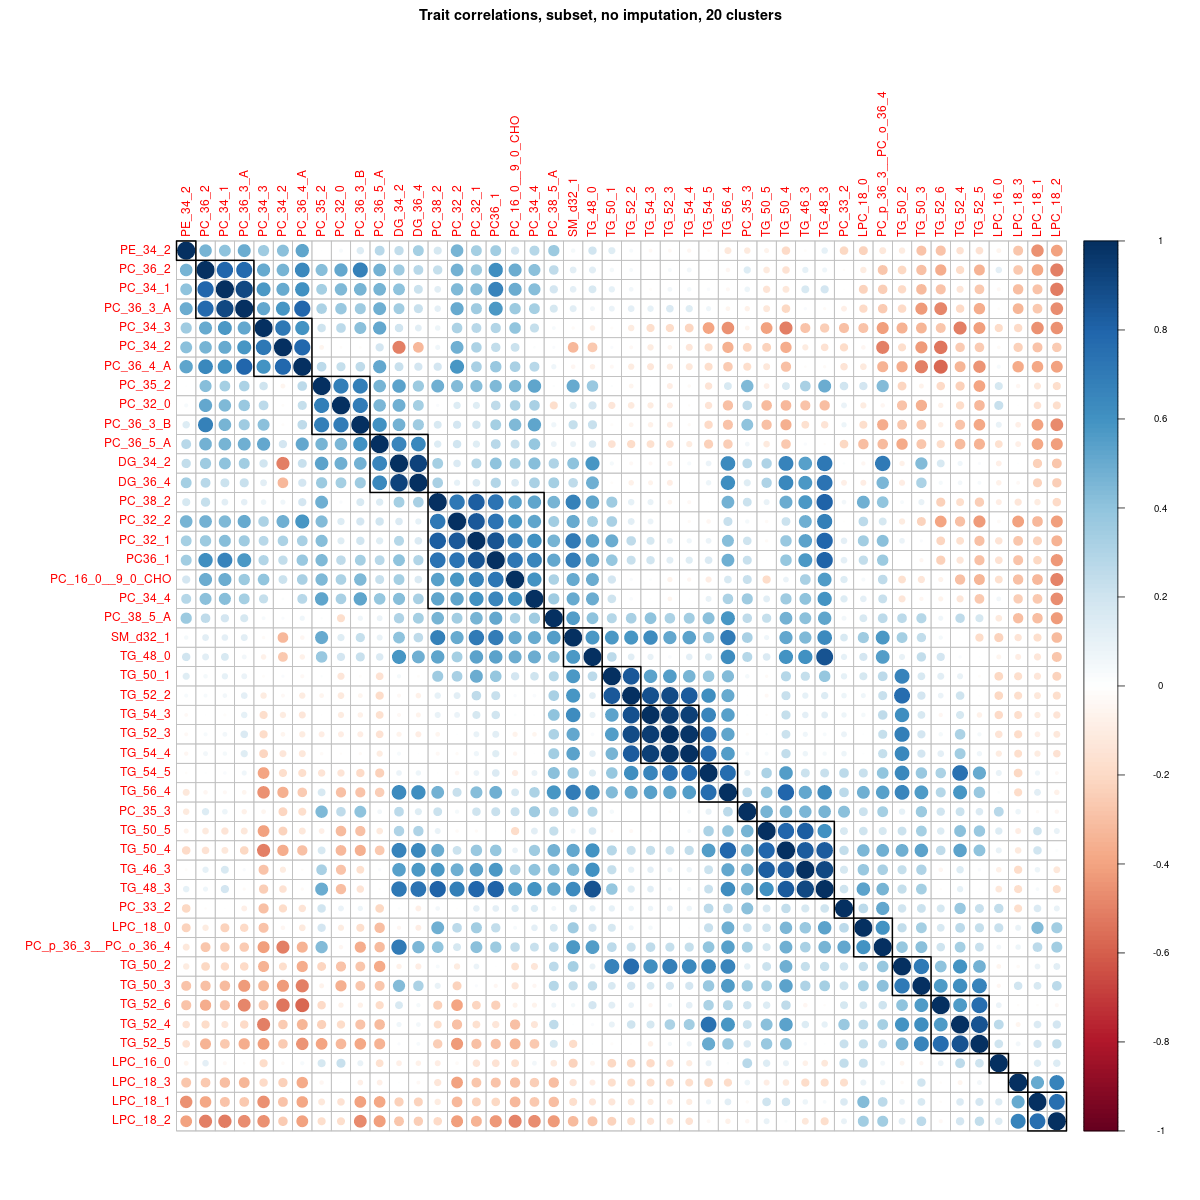
\includegraphics[width=0.9\paperwidth]{Sup_Figures/Sup_Fig_1.png}
\caption{\textit{Pcadapt} analysis of Mexican landraces. We used GBS data from the Mexican landraces of the SeeD dataset \cite{Romero_Navarro2017-cn} and run a \textit{pcadat} analysis \cite{Luu2017-ws} that identified \textbf{A)} elevation as the major driver of population differentiation, separated along Principle Component 1 (PC1).  
\textbf{B)} Genome-wide analysis of \textit{Pcadapt} PC1 outliers. 
\textbf{C)} Population Branch Excess (PBE) Analysis of genes in glycerolipid pathways.
Empirical p-value for the observed mean PBE of SNPs in genes annotated with CornCyc glycerolipid pathways. Null distribution calculated from random sampling (without replacement, 10000 replicates) of an equivalent number of SNPs in protein coding genes.
\textbf{D)} Highland selection of glycerolipid-related pathways using PBE. See methods for details.
For each pathway, we first selected all SNPs in the coding regions and 10 kb upstream and downstream of each gene to calculate the mean pathway PBE score. 
We then constructed a null distribution by drawing 10,000 samples without replacement of $n$ SNPs from those found within or around 10 kb upstream and downstream of all protein-coding genes and we obtained the mean PBE for this null distribution. 
For each pathway, the heat map shows p-values corresponding to the probability of sampling from the null distribution a set of $n$ SNPs with the observed glycerolipid-related pathway mean PBE score or higher. 
}
\label{SupFig1}
\end{center}
\end{figure*} 

\clearpage

\begin{figure*}[t]
\begin{center}
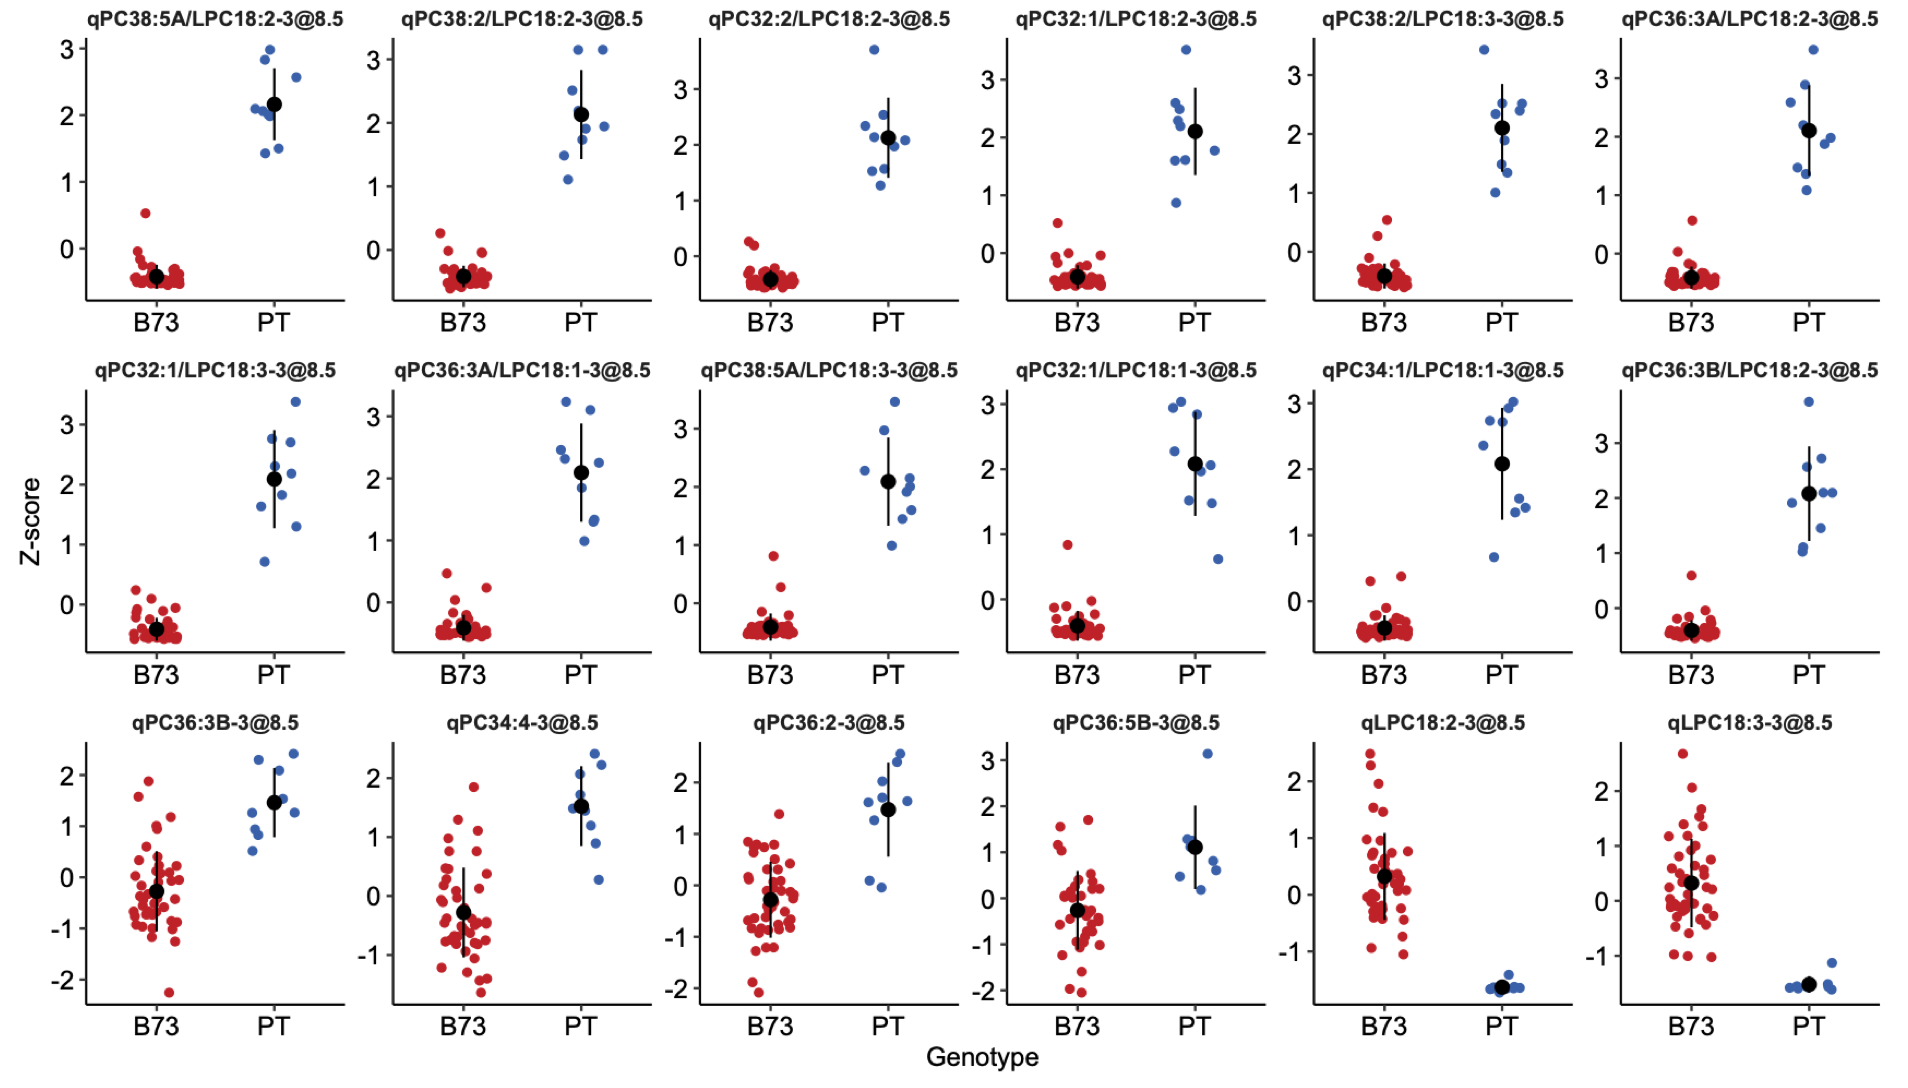
\includegraphics[width=0.9\paperwidth]{Sup_Figures/Sup_Fig_2.png}
\caption{Effects of QTLs at chromosome 3 @8.5 Mb for individual PC and LPC species (bottom), and PC/LPC ratios (12 most significant peaks).
}

\label{SupFig2}
\end{center}
\end{figure*} 

\clearpage

\begin{figure}[t]
\begin{center}
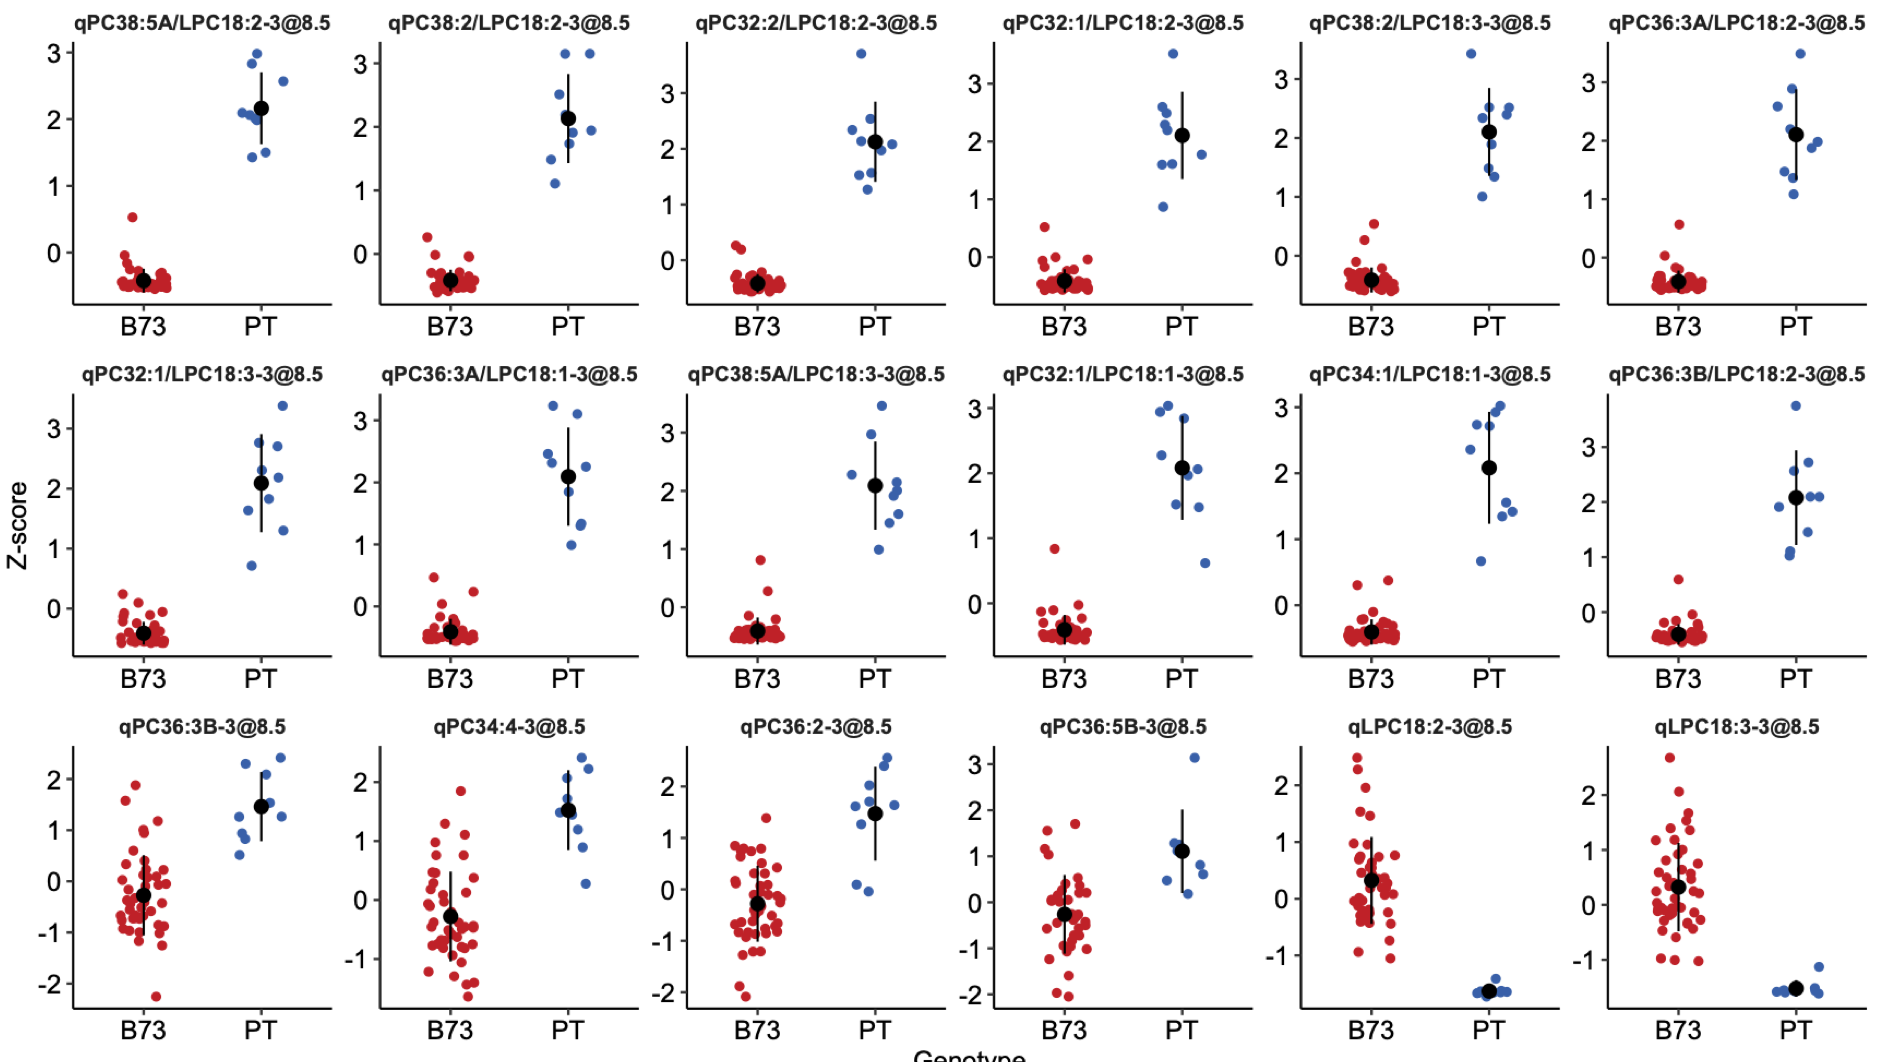
\includegraphics[width=0.4\paperwidth]{Sup_Figures/Sup_Fig_3.png}
\caption{\textbf{A)} GenomiclLocation of genes encoding proteins with predicted phospholipase A1 activity. 
\textbf{B)} Site of action of the different types of phospholipases.
\textbf{C)} Effect sizes of PC/LPC levels at RILs homozyzogous for B73, PT or heterozygous at the QTL qPC/LPC3@8.5.
} 
\label{SupFig3}
\end{center}
\end{figure}  


\clearpage

\begin{figure}[t]
\begin{center}
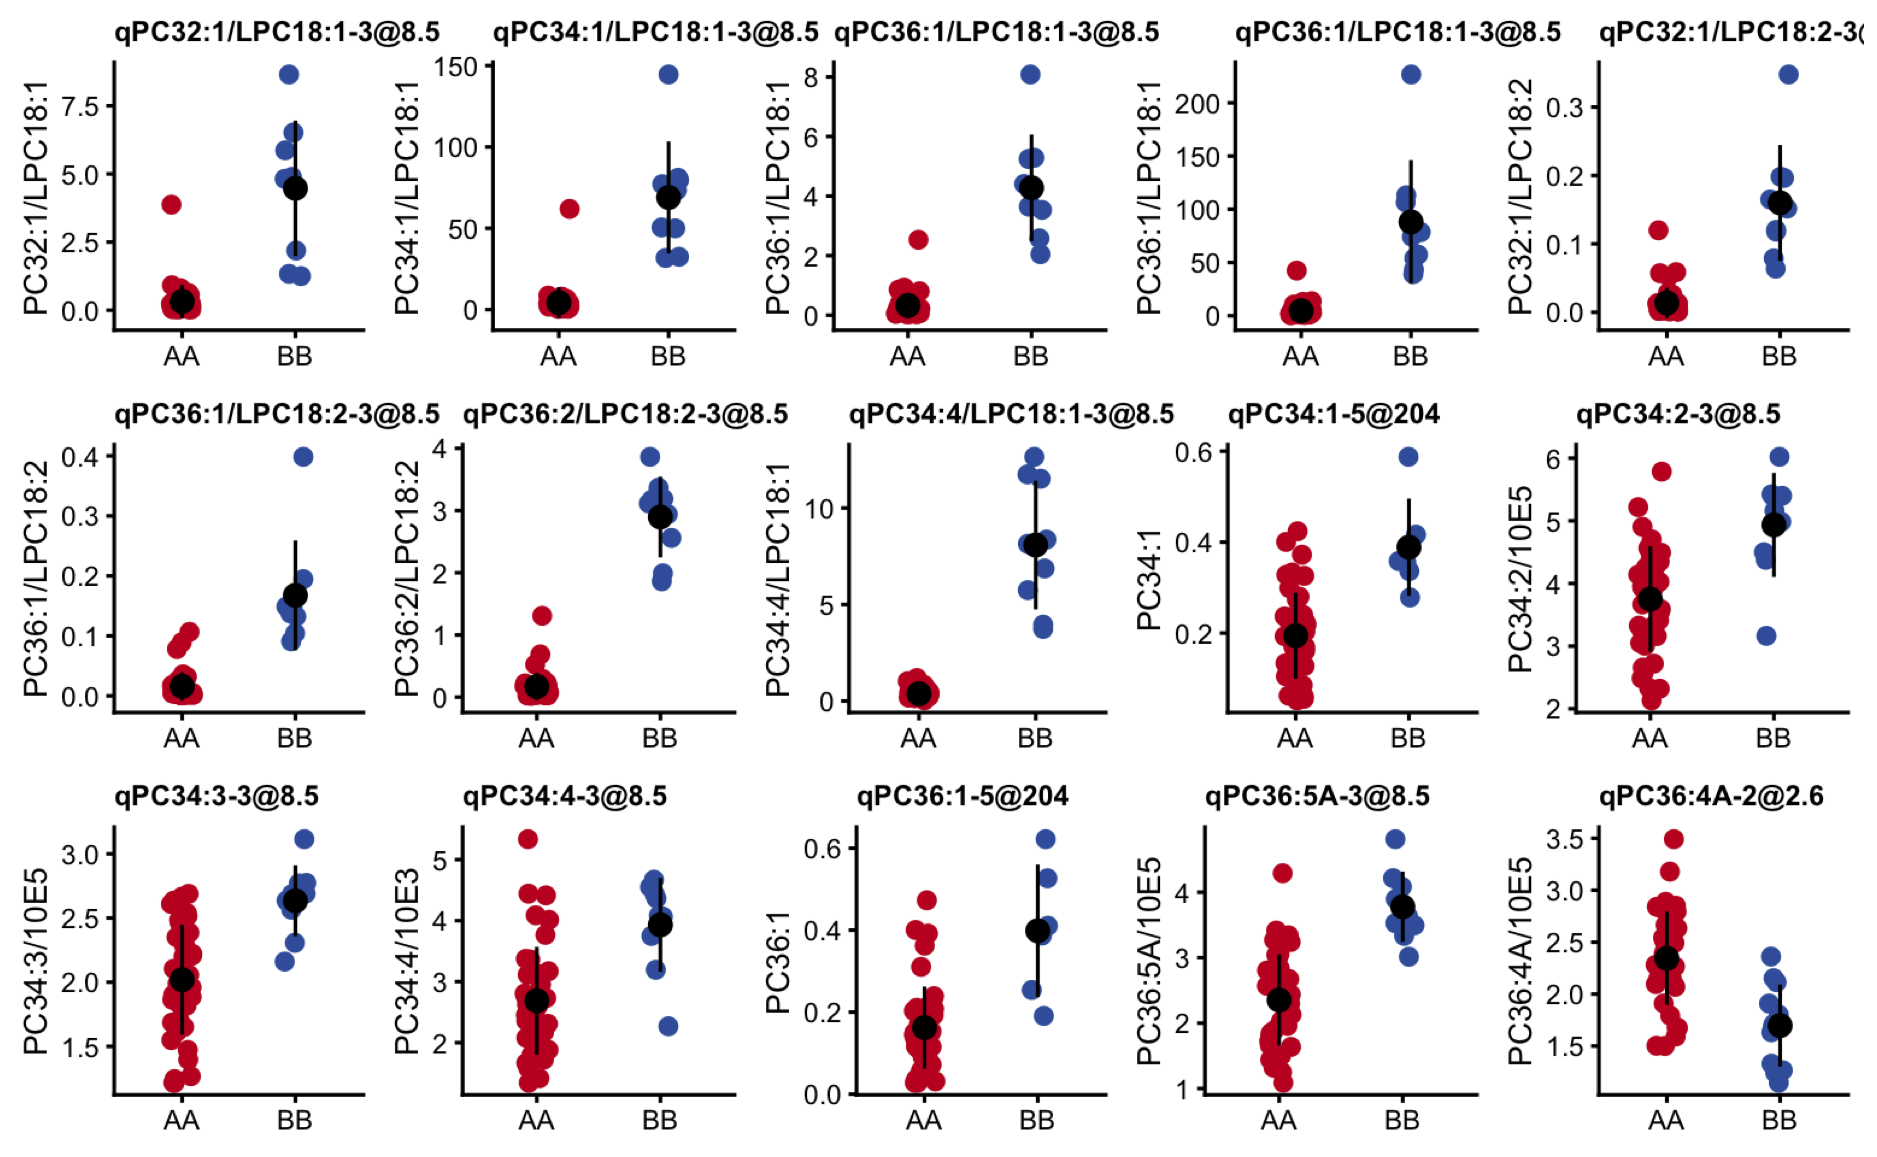
\includegraphics[width=0.6\paperwidth]{Sup_Figures/Sup_Fig_4.png}
\caption{\textbf{Subcellular localization of HPC1 in \textit{Nicotiana benthamiana} epidermal leaf cells.}   
CTP.HPC1-GFP, corresponding to the first 52 amino acids HPC1, were fused to GFP. 
Three constructs for various subcellular compartments were used as control; cytoplasm (C-GFP), nucleus (N-GFP), and chloroplast (P-GFP). All reporters were under the control of the cauliflower Mosaic Virus (CaMV) 35S promoter. The white arrows show chloroplast and nucleus.
}
\label{SupFig4}
\end{center}
\end{figure} 

\begin{figure}[t]
\begin{center}
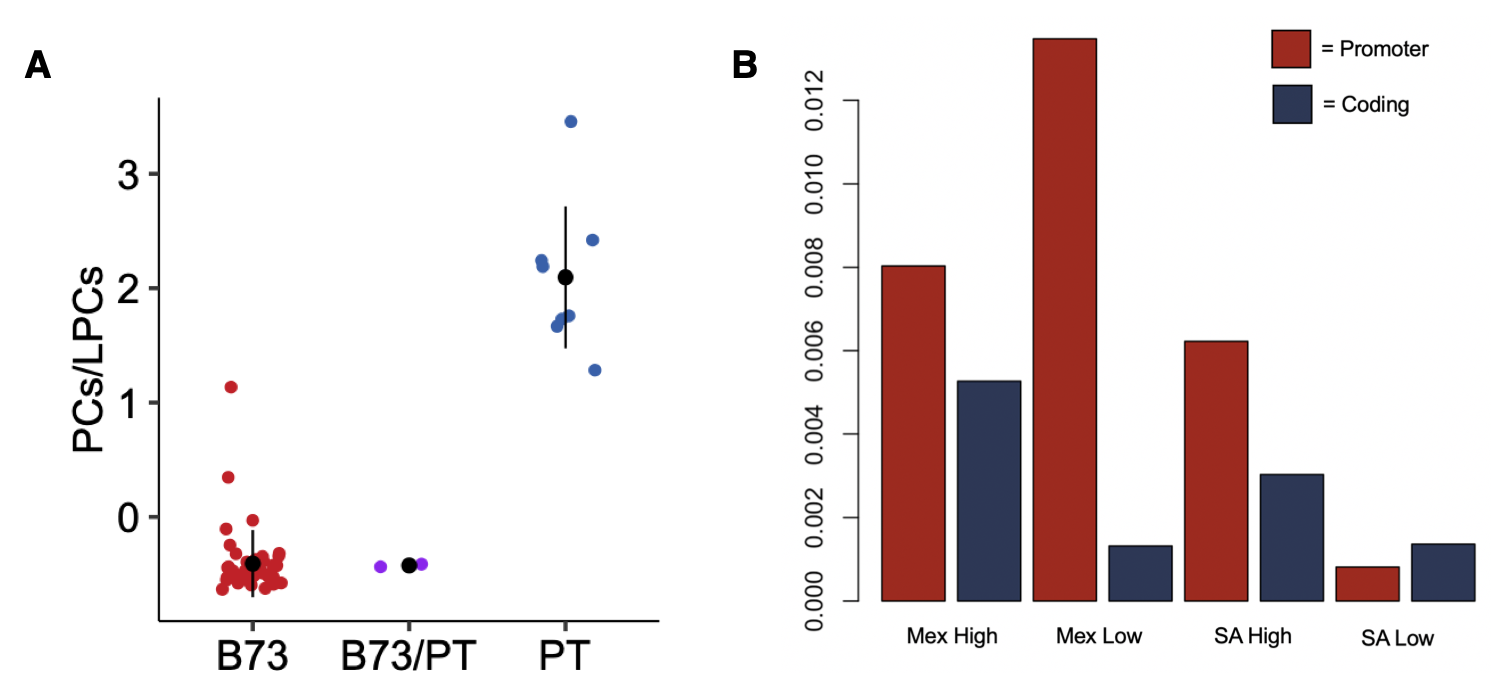
\includegraphics[width=0.8\paperwidth]{Sup_Figures/Sup_Fig_5.png}
\caption{\textbf{A)} Expression levels in B73 of genes encoding enzymes with predicted phospholipase A1 activity across different tissues. \textit{HPC1} is indicated in blue. 
Data from \cite{Stelpflug2016-vr}.
\textbf{B)} Expression levels from B73 leaves for genes in the 7.9--10 Mb QTL interval of chromosome 3. 
Data from \cite{Stelpflug2016-vr}.
\textbf{C)} \textit{HPC1} expression levels in the temperate inbred lines B73, Mo17, OH43, and PH207 under cold, control and heat stress conditions. Values taken from \cite{Waters2017-nat}
} 
\label{SupFig5}
\end{center}
\end{figure} 

\clearpage

\begin{figure*}[t]
\begin{center}
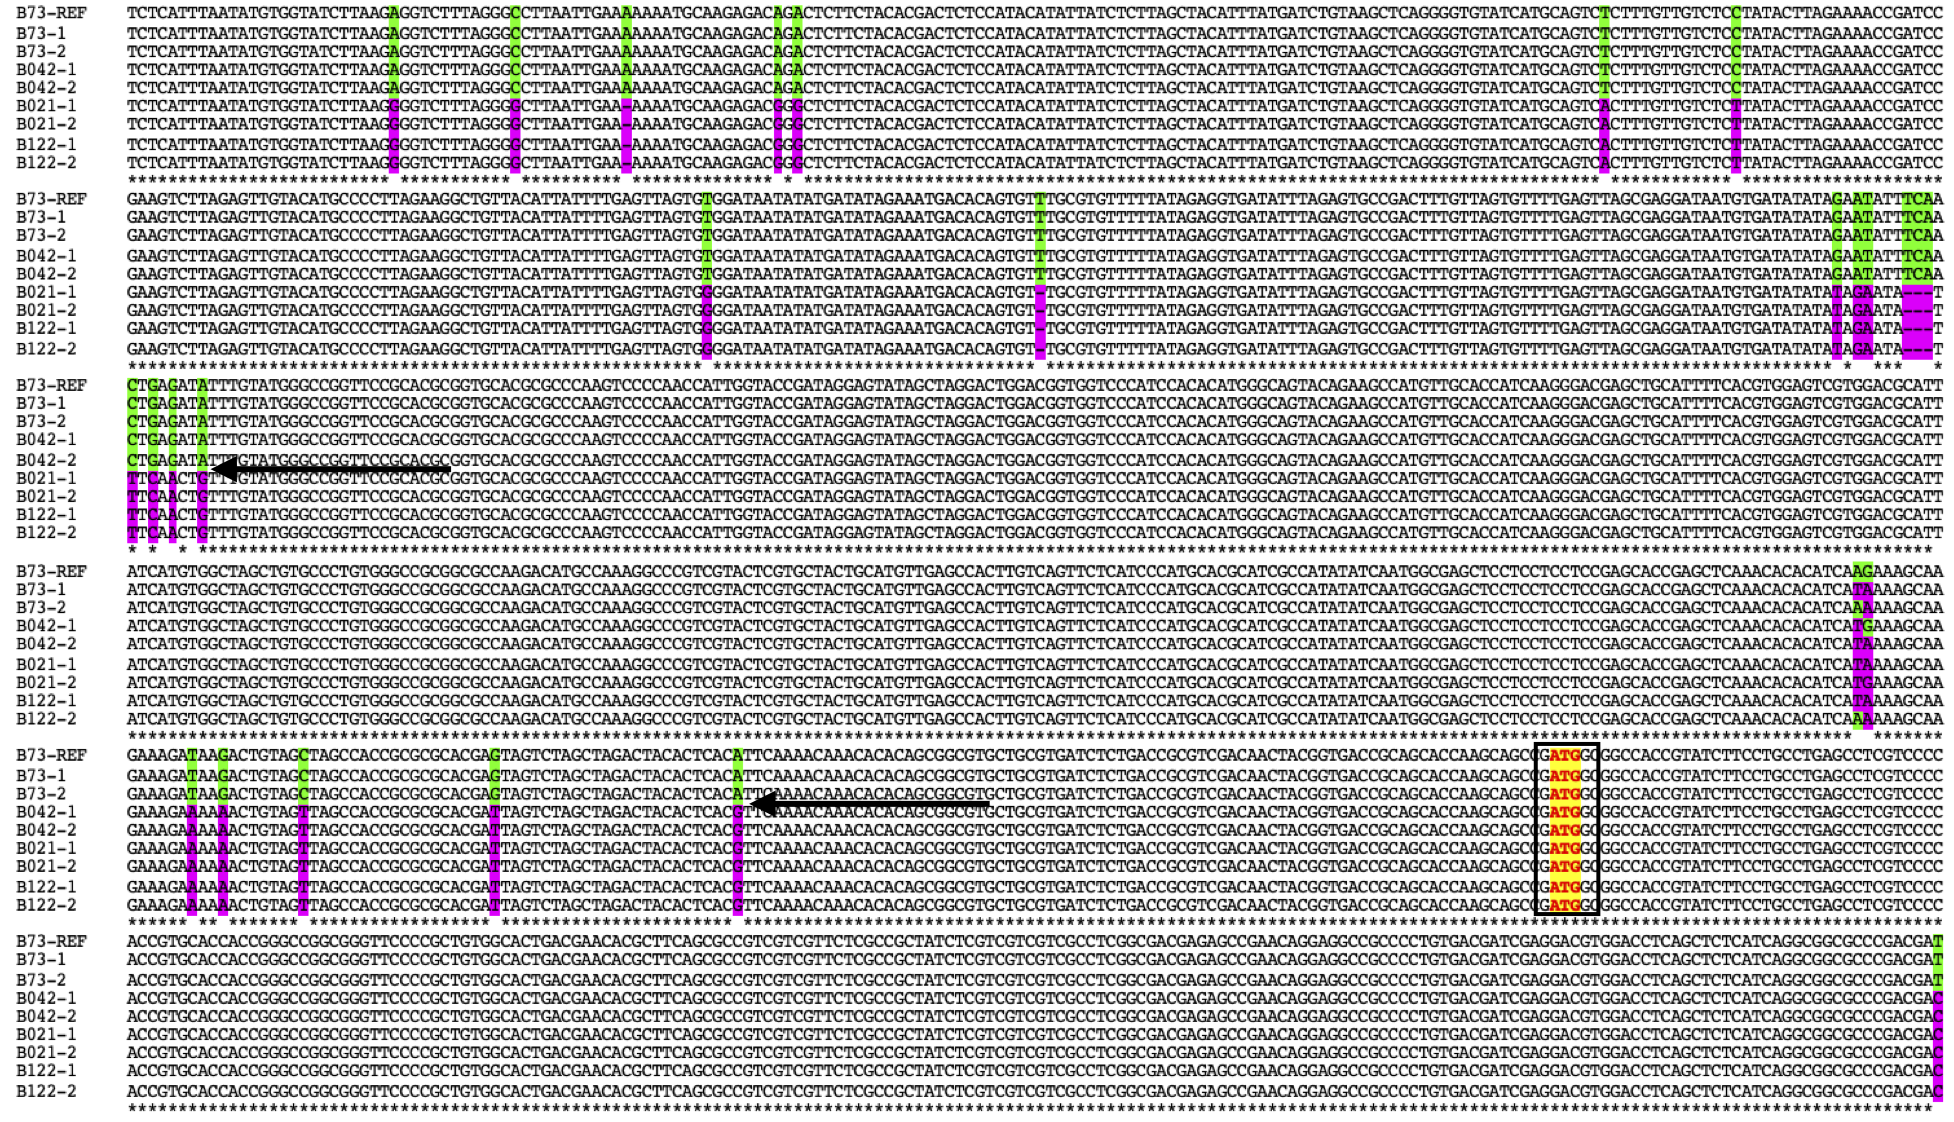
\includegraphics[width=0.9\paperwidth]{Sup_Figures/Sup_Fig_6.png}
\caption{Sanger sequencing of the promoter and start of the \textit{HPC1} genomic region obtained from B73 plants and 3 RILs (B042, B021 and B122). A recombination point 500 bp upstream the translation start codon in B1042 is indicated by arrows. B73 alleles are marked in green and PT alleles are marked in pink. 
}
\label{SupFig6}
\end{center}
\end{figure*} 


\clearpage

\begin{figure*}[t]
\begin{center}
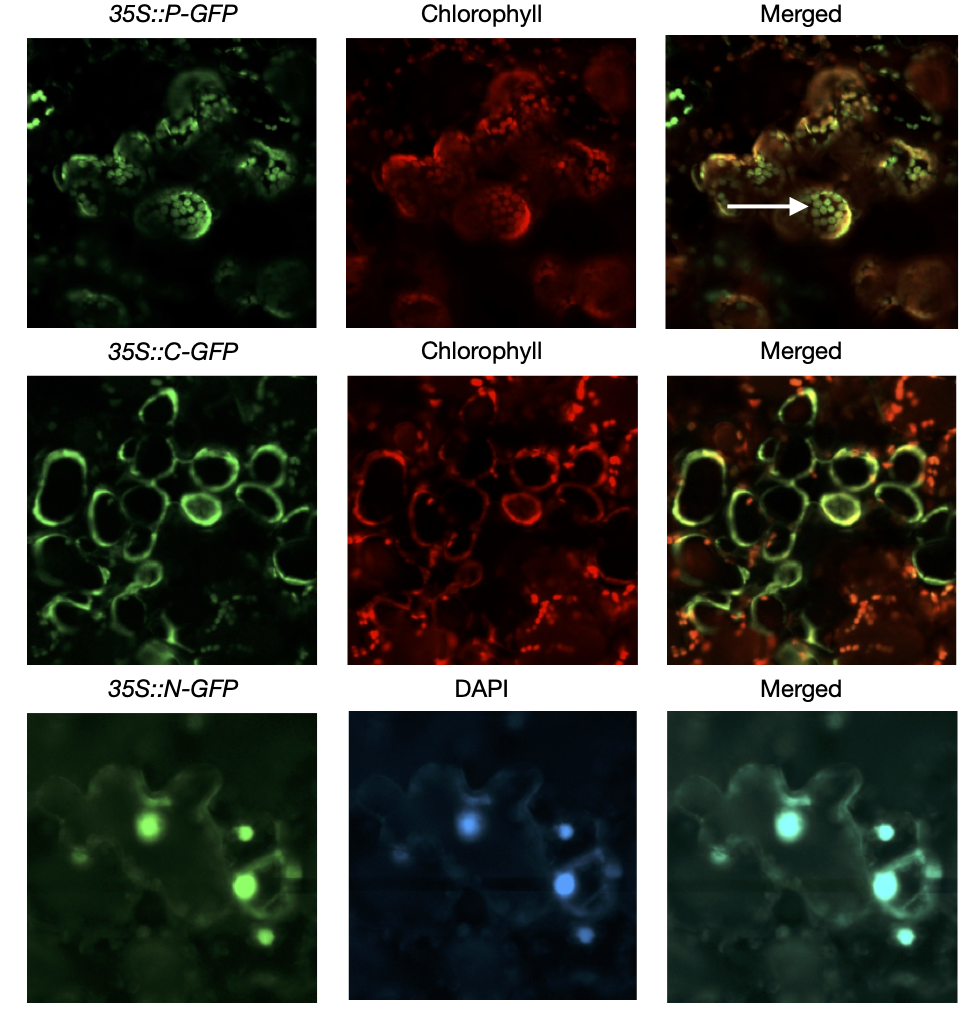
\includegraphics[width=0.8\paperwidth]{Sup_Figures/Sup_Fig_7.png}
\caption{B73 and PT HPC1 proteins aligned using ClustalOmega. 
Green residues are those from the chloroplast transit peptide. Blue resides are part of the Lipase3 domain. 
Magenta residues are the flap lid. 
Arrow denotes I211V mutation. “*” denotes matching sequence, “:” denotes conservation between groups with similar properties, “.” denotes conservation of groups with weakly similar properties. 
}
\label{SupFig7}
\end{center}
\end{figure*} 


\clearpage

\begin{figure*}[t]
\begin{center}
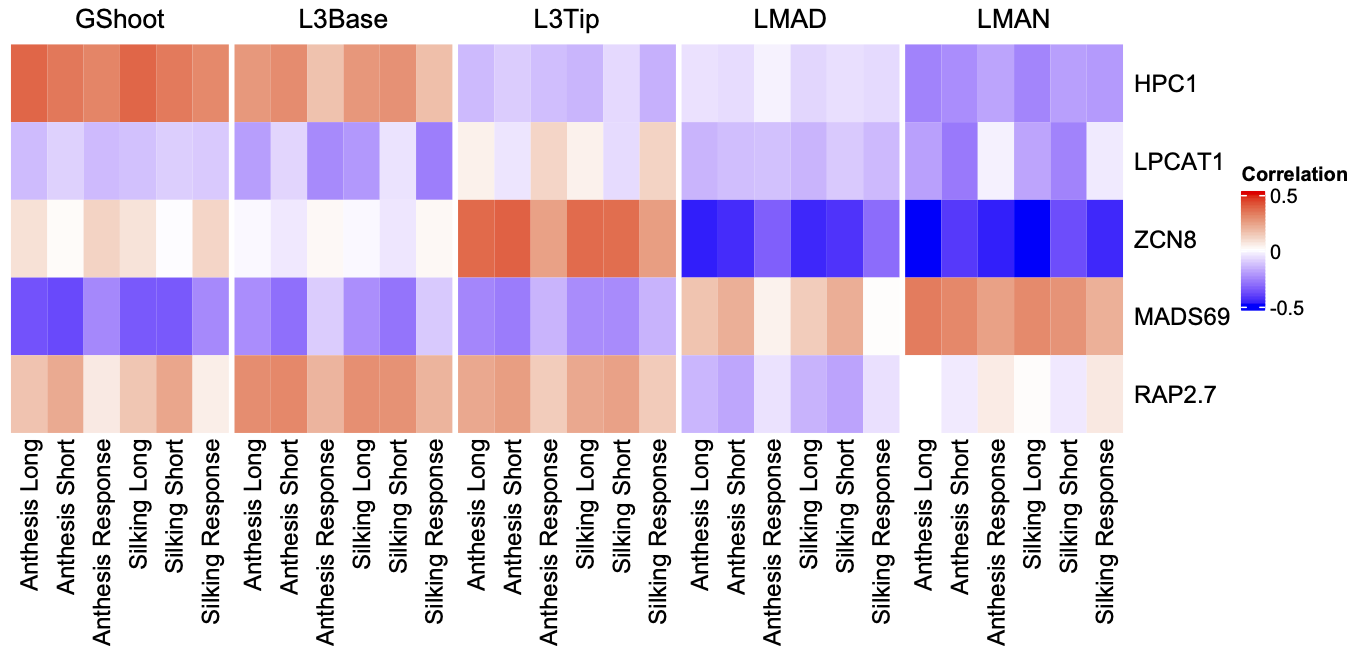
\includegraphics[width=0.8 \paperwidth]{Sup_Figures/Sup_Fig_8.png}
\caption{Correlation between flowering time and expression of phospholipid-related genes, using flowering time traits from aerial tissues in the 282 diversity panel. 
Data obtained from \cite{Kremling2018-gn}}.
\label{SupFig8}
\end{center}
\end{figure*} 

\clearpage
\end{document}
